\cotefile{136}
\scanpage{48}
\margin{\uline{\unsure{Cohomologie} des ens. $\frac12$ \unsure{simpliciaux}
et \unsure{résolutions can.} $\frac12$ \unsure{simpliciales}}}

Soit $k$ un \deleted{groupe abélien}\inserted{\unsure{anneau}}, $M$ un $k$-module,
\[
C^*:\widehat{\Delta}^{\circ}\longrightarrow
\text{\unsure{complexes croissants} de $k$-modules}
\]
un foncteur \unsure{contravariant} tel que

a) $\forall X_*\in\operatorname{Ob}\widehat{\Delta}$,
$\unsure{H^*(X_*^\vee,M)}\simeq H^*(C^*(X_*))$.
(\unsure{isom. fonctoriel} en $M$ --- \unsure{au minimum} pour $H^0$)

b) $\forall n\geq 0$, $X_*\longmapsto C^n(X_*)$
\unsure{transforme} $\unsure{\underset{\longrightarrow}{\lim}}$ en
$\unsure{\underset{\longleftarrow}{\lim}}$.

Alors b) signifie que les $C^n$ sont \unsure{représentables}
\[
C^n(X_*)=\operatorname{Hom}(X_*,C_*^n).
\]
a) implique, en \unsure{faisant} $X_*=\unsure{\Delta_n}$, que les
$C_n^*$ sont des \uline{résolutions} de $M$, \unsure{alors que l'augmentation}
$M\longrightarrow C_n^*$ est \unsure{fonctorielle} en $\unsure{\Delta_n|M}$.
$C_*^*$ est une résolution de
$\unsure{M_*=\mathbf Z_*\otimes M\simeq M_{\Delta_*}\otimes M}$,
ce qui implique bien que \unsure{l’on a un morphisme canonique}
$\unsure{H^*(C^*(X_*))\simeq H^*(X_*,M)}$,
\illegible{4} \unsure{fonctoriel}.
\margin{\unsure{Ceci est déjà} \illegible{2}!}

En prenant $X_*=\unsure{\Delta_n}$ \unsure{contractile}, on \illegible{3}
que $\unsure{H^i}$ \illegible{4}
($\unsure{H^0(C^*(X_*))=M}$).
\unsure{Pour} $\uline{\unsure{H^1}}$ \illegible{4} \unsure{pour}
$\unsure{C_*^*}$ \illegible{2}
\unsure{(analogue à} $\unsure{M_*}$\unsure{)}, i.e.
\illegible{2} $X_*\longrightarrow\unsure{Z_*^i}$

\diagram{\begin{tikzcd}
\unsure{C_*^{i-1}} \arrow[r] & \unsure{Z_*^i}\\
& X_* \arrow[u]
\end{tikzcd}}
(\unsure{pour}
\diagram{\begin{tikzcd}
C_*^0 \arrow[r] & Z_*^1\\
& X_* \arrow[u]
\end{tikzcd}})

\unsure{Si l'on} \illegible{1} $\unsure{C_*^{i-1}}$ \illegible{2},
\unsure{on n'a} \illegible{3}
\unsure{a) que les prolongements} \illegible{1} \unsure{pour les}
$C_*^i$ \unsure{sont flasques},
(\unsure{ce qui est} \illegible{1} \unsure{pour} \illegible{3}).

\deleted{\unsure{À supposer} \illegible{4} \unsure{qu'on} \illegible{2}
\unsure{pour} \illegible{1},
\unsure{fonctoriel} \illegible{4} $\unsure{C_*^i}$. On aura
\[
\unsure{H^0(X_*,C_*^0)}
\unsure{\longrightarrow}
\unsure{H^0(X_*,Z_*^1)}
\longrightarrow \unsure{H^1(X_*,M)}
\longrightarrow \unsure{H^1(X_*,C_*^0)}
\longrightarrow \unsure{H^1(X_*,Z_*^1)}.
\]
\inserted{\unsure{épim.} a)}\inserted{\unsure{inj.}}}

Mais c'est \unsure{faux déjà pour} $M=0$.
\unsure{Ceci suffit}, \unsure{pour que}, \illegible{1} b),
\unsure{que le} \illegible{2} \unsure{en} $\unsure{C_*^0\longrightarrow C_*^1}$,
\unsure{splittings} \illegible{2}!

\uline{NB} \unsure{Supposons} $C_*^*$ une \unsure{résolution flasque de} $M_*$,
les $\unsure{Z_*^{n+1}}$ \illegible{2} \unsure{connexes},
des $\unsure{K_*(M,n)}$ \illegible{1}.
\margin{47}

\scanpage{49}
\margin{\unsure{84|48}}
\begin{flushright}6\end{flushright}

Continuing in this way we construct the minimal model
\[
\Lambda(x_1,x_2,\ldots:d)\underset{\rho}{\longrightarrow}\mathcal E
\]
satisfying properties i) and ii) above.

\uline{Theorem B}: Let $X$ be a triangulated space which is simply connected. If
\[
\Lambda(x_1,x_2,\ldots)\underset{\rho}{\longrightarrow}\mathcal E
\]
is a minimal model of the de Rham algebra then

i) the rank of $\pi_i X$ is the number of variables in degree $i$.

ii) the rank of the Hurewicz homomorphism
$\pi_i X\longrightarrow H_i X$ is the number of $d$-closed generators in degree $i$.

iii) the Whitehead products on homotopy are described by the quadratic terms of the $d$-formulae of generators.

Theorem B is proved by a not so standard Postnikov argument using Theorem A and the commutativity of the wedge product multiplication in $\mathcal E$. The argument is based on the beautifully simple Guy Hirsh method of computing the cohomology of a principal $G$-bundle over a manifold using differential forms (see appendix H). The Hirsch method was suggested by Rene Thom in the study of Postnikov systems in the Cartan Seminar 1954.

The proof of theorem B shows the model can be used to directly construct the \uline{rational} Postnikov system

\scanpage{50}
\uline{Ex 1} \unsure{$n$ fixé}, \unsure{prenons le foncteur} \unsure{donné par}
$\unsure{u_n^*(K)=K_n}$.
\[
M\longmapsto C^n(K_*,M)\overset{\unsure{\mathrm{d\acute{e}f}}}{=}
\operatorname{Hom}_{\unsure{\mathrm{Ens}}}(K_n,M)
=\operatorname{Hom}_{\unsure{\mathrm{Ens}}}(\unsure{u_n^*(K)},M)
\simeq \operatorname{Hom}_{\widehat{\Delta}}(K_*,\unsure{u_{n*}(M)}).
\]
\unsure{est représentable par} $\unsure{u_{n*}(M)}$.
\unsure{Puis, naturellement, les} $\unsure{u_{n*}(M)}$
forment un $k$-Module \unsure{cosimplicial} de $\widehat{\Delta}$, d'où
(\unsure{en passant au complexe} \illegible{3})
un complexe de \unsure{cochaînes} de $k$-Modules, qui est
$\unsure{C_{*M}^*}$. \unsure{D'où}
\[
C^*(K_*,M)\simeq\operatorname{Hom}(K_*,C_{*M}^*).
\]
(\unsure{Isom.}, \unsure{au choix}, de $k$-Modules \unsure{cosimpliciaux},
\unsure{ou de complexes de cochaînes}, \illegible{3} \unsure{le complexe} $K$).

On sait que pour $K_*=\Delta_n$, on a une \unsure{résolution}
de $M$, \unsure{donc} $C_{*M}^*$ est une résolution de $M_*$.
De plus les $\unsure{C_{*M}^n=u_{n*}(M)}$ sont \unsure{flasques},
\illegible{3}, $M$ \unsure{un} \illegible{1}!
\margin{NB $\unsure{C_{nM}^p=u_{p*}(M)_n
=\operatorname{Hom}(\Delta_n,\Delta_p)\cdot M
=M^{\operatorname{Hom}(\Delta_n,\Delta_p)}}$
$\unsure{=k^{\operatorname{Hom}(\Delta_n,\Delta_p)}\otimes_k M}$}

\uline{Ex 2} \unsure{Considérons le sous-complexe de cochaînes}
du $k$-Module \illegible{1} $C_{*M}^*$, formé des \unsure{cochaînes}
\unsure{non dégénérées}:
\[
\unsure{C_{*M}^{*!}=(C_{*M}^{n!})_{n\geq0}}:
\]
\[
\begin{aligned}
\unsure{C_{*M}^{n!}}
&=\bigcap_{\substack{\unsure{\sigma:\Delta_n\to\Delta_m}\\
\unsure{\sigma\text{ ép.},\,m<n}}}
\operatorname{Ker}(\sigma:C_{*M}^n\longrightarrow C_{*M}^m)\\
&=\bigcap_{\substack{\unsure{u_i:\Delta_n\to\Delta_{n-1}}\\
\unsure{i<n}}}
\operatorname{Ker}(\unsure{u_i}:C_{*M}^n\longrightarrow C_{*M}^{n-1})\\
&=\bigcap_{\substack{\unsure{\sigma:\Delta_n\to\Delta_m}\\
\unsure{m<n,\ \text{quelconque}}}}
\operatorname{Ker}(\sigma:C_{*M}^n\longrightarrow C_{*M}^m).
\end{aligned}
\]
On sait que cette \unsure{opération} \unsure{fournit} \illegible{4}
\unsure{un complexe} \illegible{2} \unsure{qui donne} \illegible{3}
\unsure{de} \illegible{3} \unsure{par} \illegible{2}
$\unsure{C^{*!}(X_*)\subset C^*(X_*)}$.
\margin{49}

\scanpage{51}
\margin{\unsure{50|05}}
\begin{flushright}5\end{flushright}

algebra of $X$ \uline{\unsure{(in any sense), then one finds the second homotopy group}}
$\pi_2X$ has rank $n$, $\pi_3X$ has rank $\ell+m$, the Hurewicz map
$\pi_3X\longrightarrow H_3X$ has rank $\ell$, and the symmetric pairing given by Whitehead product
\[
\pi_2X\otimes\pi_2X\xrightarrow{[\ ,\ ]}\pi_3X
\]
is described over the rationals by the $i,j$ symmetric tensor $(a^k_{ij})$.)

Now suppose by induction that
\[
\Lambda(x_1,\ldots,x_n;y_1,y_2,\ldots;z_1,z_2,\ldots:d)
\xrightarrow{\rho_n}\mathcal E
\]
has been constructed so that $d$ of any generator is a polynomical in previous generators while $\rho_n$ is an isomorphism on cohomology up through dimension $n$ and injective in dimension $n+1$.

Then as in step 2 we adjoin variables in dimension $n+1$ to make $\rho$ onto in dimension $n+1$ and injective in dimension $n+2$. In this general case we add variables
$\omega_1,\ldots,\omega_d,\omega_{d+1},\ldots,\omega_r$
and define $d$ and $\rho=\rho_{n+1}$ as above.
Now $d\omega_1,\ldots,d\omega_d$ are zero and
$\rho\omega_1,\ldots,\rho\omega_d$ give generators of the cokernel of $\rho_n$ on $H^{n+1}$,
$d\omega_{d+1},\ldots,d\omega_r$ are polynomials in
$x_1,x_2,\ldots;y_1,y_2,\ldots;z_1,z_2,\ldots$
which generate the kernel of $\rho_n$ on
\[
H^{n+2}(\Lambda(x_1,x_2,\ldots;y_1,y_2,\ldots;z_1,z_2,\ldots:d))
\]
and $\rho\omega_{d+1},\ldots,\rho\omega_r$ are elements in $\mathcal E$ whose differentials are these same polynomials in
\[
\rho x_1,\rho x_2,\ldots;\rho y_1,\rho y_2,\ldots;\rho z_1,\rho z_2,\ldots\,.
\]

\scanpage{52}
\unsure{vu que l'opération} \unsure{de passage au sous-complexe des}
\unsure{cochaînes non dégénérées commute à}
$\operatorname{Hom}(X_*,-)$.
Donc
$\unsure{C^{*!}(X_*)=\operatorname{Hom}(X_*,C_{*M}^{*!})}$
\unsure{satisfait encore aux conditions} a) et b).
\unsure{D'autre part, les} $\unsure{C_{*M}^{n!}}$ \unsure{sont flasques},
\unsure{en effet, on} \unsure{explicite} \unsure{aisément}
\[
\begin{aligned}
\unsure{(C_{*M}^{n!})_m}
&\simeq M^{\unsure{\operatorname{Hom}_{\mathrm{mono}}(\Delta_n,\Delta_m)}}
\simeq k^{\unsure{\operatorname{Hom}_{\mathrm{mono}}(\Delta_n,\Delta_m)}}\otimes_k M\\
&\simeq \bigl(\textstyle\bigwedge^{n+1}k^{\Delta_m}\bigr)\otimes_k M.
\end{aligned}
\]
\unsure{et cette formule} \illegible{4}, d'où
\[
\unsure{C_{*M}^{n!}\simeq\bigwedge^{n+1}\Phi_{*k}\otimes_k M}
\]
où $\unsure{\Phi_{*k}=(\Delta_*\longmapsto k^{\Delta_*})}$.
[\unsure{les} \illegible{2} \unsure{des} \illegible{1}

\unsure{Soit} \illegible{2}
\[
\unsure{T:k_*\longrightarrow \Phi_{*k}=C_{*k}^{0!}}
\]
\illegible{2} \unsure{est la coaugmentation}
($\unsure{\Phi_{-1,k}=k}$).

\unsure{Alors} \unsure{l'opérateur différentiel} \unsure{s'identifie},
\unsure{donc}
$\unsure{C_{*M}^{n!}\simeq\bigwedge^{n+1}\Phi_{*k}\otimes_k M}$
\unsure{étant muni} \unsure{par} $\unsure{T\wedge}$.
\unsure{C'est} \unsure{une formule commode} \unsure{pour calculer les} \illegible{1}].
\unsure{Or} \illegible{2} \unsure{lorsque} \illegible{2}
\unsure{particulier}, \illegible{3},
$\unsure{\bigwedge^i \Phi_{*k}\otimes_k M}$.
\illegible{3} $\unsure{\bigwedge^0\Phi_{*k}\otimes_k M}$,
\illegible{3} \unsure{de} \illegible{2}.

\unsure{On retrouve en même temps les propriétés de}
$\unsure{C_{*k}^{*!}}$:
\unsure{c'est un complexe de} \unsure{groupes abéliens|foncteurs ab.},
\illegible{3}
\unsure{dont} \illegible{1} (\unsure{savoir pour les}
\illegible{2} \unsure{les})
\unsure{une structure} \illegible{2}
$\unsure{\partial:C_{*M}^n\longrightarrow C_{*M}^{n+1}}$
\illegible{2} (\unsure{sauf erreur}).
\margin{51}

\scanpage{53}
\margin{\unsure{52|25}}
\begin{flushright}4\end{flushright}

Suppose always that $\mathcal E$ is homologically connected and for the moment that the first Betti number of $\mathcal E$ is zero.

\uline{Step 1}: Construct $\Lambda(x_1,\ldots,x_n)\xrightarrow{\rho_1}\mathcal E$ where $x_1,\ldots,x_n$ are in dimension 2 and $\rho_1x_1,\ldots,\rho_1x_n$ generate $H^2\mathcal E$.
Define $d$ in $\Lambda(x_1,\ldots,x_n)$ by $dx_i=0$, $i=1,\ldots,n$.
Note that $\rho_1$ is an isomorphism on cohomology in dimension 2 and injective in dimension 3.

\uline{Step 2}: Adjoin three-dimensional variables to $\Lambda(x_1,\ldots,x_n)$ to make $\rho_1$ surjective on cohomology in dimension 3 and injective on cohomology in dimension 4.

More explicitly, we form
\[
\Lambda(x_i;y_j),\ \rho_2,\ \text{and }d.
\]
$d$ is defined by
\[
\begin{aligned}
dy_1&=0,\ldots,dy_\ell=0\\
dy_{\ell+k}&=\sum a^k_{ij}x_i\wedge x_j
\qquad k=1,\ldots,m
\end{aligned}
\]
\figure{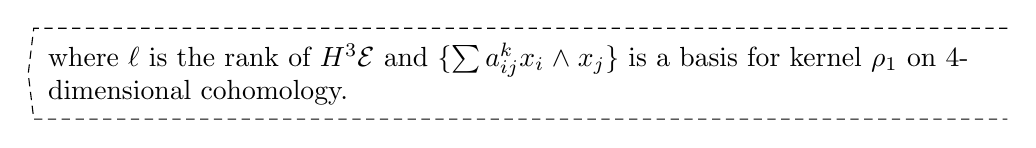
\begin{tikzpicture}
\node[anchor=north west,text width=12cm,inner sep=5pt] (p) at (0,0)
{where $\ell$ is the rank of $H^3\mathcal E$ and
$\{\sum a^k_{ij}x_i\wedge x_j\}$ is a basis for kernel $\rho_1$ on 4-dimensional cohomology.};
\draw[densely dashed] (p.north east)--(p.north west)--([xshift=-2pt]p.west)--(p.south west)--(p.south east);
\end{tikzpicture}}

$\rho_2$ is defined by choosing $\rho_2y_1,\ldots,\rho_2y_\ell$ to generate $H^3\mathcal E$ and $\rho_2(y_{\ell+k})$, $k=1,\ldots,m$, to satisfy
\[
d(\rho_2(y_{\ell+k}))=\sum_{i,j}a^k_{ij}\rho_1(x_i)\wedge\rho_1(x_j).
\]
(Now $\rho_2$ is an isomorphism on $H^3$ and injective on $H^4$.

At this point one can show by a standard Postnikov argument how this construction relates to the homotopy theory of a simply connected space $X$. If $\mathcal E$ is the de Rham

\scanpage{54}
\uline{Intégration des algèbres $\frac12$ simpliciales}

Soit $A_*$ un groupe gradué différentiel $\frac12$ simplicial
i.e. un objet $\frac12$ simplicial dans la catégorie des groupes
gradués différentiels (: op. de dérivation de degré $+1$).
\deleted{On suppose} Donc $\forall n\geq0$
\[
A_n=A_n^*=\sum_{p\in\mathbf Z}A_n^p,
\]
avec op. différentielle
$d_n:A_n^*\mathbin{-}A_n^*$,
$A_n^p\mathbin{-}A_n^{p+1}$.
On suppose

\margin{\figure{\begin{tikzpicture}\draw (0,0)--(0,-3.2);\end{tikzpicture}}}
(1) $\forall n,\ n\geq0\quad A_n^p=0$ si $p\notin[0,n]$,
et \deleted{\unsure{le}} $A_n^*$ muni
de l'augmentation \inserted{$\unsure{\varepsilon_n}:$}
$A_0\longrightarrow A_n^*$
[\uline{NB} associée à l'unique $\sigma:\Delta_n\longrightarrow\Delta_0$;
$A_0$ est considéré comme groupe \unsure{muni de la}
graduation nulle et l'op. diff. trivial]
est une \uline{résolution} de $A_0$.

Rappelons qu'on a sur le système des $A_n$ un op.
différentiel (i.e. de degré $-1$)
\[
\partial:A_n^*\mathbin{-}A_{n-1}^*
\]
\[
\partial(\omega)=\sum_{0\leq i\leq n}\partial_{n,i}^*(\omega)(-1)^i
\]
(où les $\partial_{n,i}$, $(0\leq i\leq n)$ sont les \unsure{$n+1$ applications}
strictement croissantes $\Delta_{n-1}\mathbin{-}\Delta_n$.
On sait que $\partial(\partial\omega)=0$.

\uline{Proposition 1} Il existe un et un seul système d'hom.
de groupes
\[
A_n^*\xrightarrow{\unsure{K_n|k_n}}A_0
\]
satisfaisant aux conditions suivantes
\margin{\figure{\begin{tikzpicture}\draw (0,0)--(0,-2.1);\end{tikzpicture}}}
\margin{\uline{NB} le système des $K_n$ \uline{ne commute pas}
en \unsure{gén.} aux op. $\frac12$ simpliciales!}

a) (normalisation) $\quad K_0=\operatorname{id}_{A_0}$

b) (condition de degré) $\quad K_n(A_n^p)=0$ si $p\ne n$

c) (Stokes) $\quad K_n(d\omega)=K_{n-1}(\partial\omega):
\ \forall\omega\in A_n^*$.

En vertu de b), la condition c) équivaut à la même
condition, avec $\omega\in A_n^{n-1}$. On montre existence et
unicité par \inserted{\unsure{degré $\leq N$ par}} récurrence sur $N$,
en notant que pour $N=0$ c'est trivial.
Si $N>0$, \deleted{$\unsure{\bar\omega\in A}$}
il reste à démontrer ex. et un. de $K_N$, i.e. de
$K_N(\bar\omega^N)$ pour $\bar\omega^N\in A_N^N$.
Or $d\bar\omega^N=0$ puisque $A_N^{N+1}=0$
\inserted{(1)}, donc $\bar\omega^N=d\omega^{N-1}$ (1).
[En fait il suffit \inserted{ici} $H^N(A_N^*)=0$ pour $N\geq1$]
\unsure{on le} \uline{\unsure{définit}} par c):
\[
\unsure{K_N|K_n}(d\omega^{N-1})=\unsure{K_{N-1}|K_{n-1}}(\partial\omega)
\]
\margin{53}

\scanpage{55}
\begin{center}- 130 -\end{center}
\begin{flushright}IX\end{flushright}

Elle implique bien que si $\varphi^t_{\xi_{\unsure{o|0}}}$ est symétrique et positive, il en est de même de $\varphi^t_\xi$.

Enfin, le fait que $\varphi^t_{\xi_{\unsure{o|0}}}$ soit non dégénérée équivaut évidemment à l'assertion que l'accouplement (10.4.1) est séparant (compte tenu que
$\xi_{\unsure{ot|0t}}:M\otimes_{\mathbb Z}\mathbb Q\longrightarrow M'\otimes_{\mathbb Z}\mathbb Q$
est un isomorphisme, $\widetilde\xi_{\unsure{o|0}}$ étant une isogénie), et est donc également indépendant de la polarisation choisie. On peut d'ailleurs noter que pour vérifier que (10.4.1) est séparant, il suffit de vérifier la même assertion pour l'accouplement de monodromie $u_\ell$ (9.1.2) pour \uline{un} nombre premier $\ell$. Prenant $\ell\ne p$, on peut utiliser la description 9.2 de $u_\ell$; le fait que $u_\ell$ soit séparant à gauche (donc des deux côtés, pour une raison de rangs) est alors trivial.

11. \uline{Composantes connexes du modèle de Néron}: \uline{relation de dualité, comportement asymptotique}.

11.0. Le but du présent paragraphe est l'étude du $k$-groupe fini étale
\[
\text{(11.0.1)}\qquad
\Phi_{\unsure{o|0}}=A_{\unsure{o|0}}/A_{\unsure{o|0}}^{\unsure{o|0}}
\]
déjà considéré dans 1. Pour tout nombre premier $\ell$, nous désignons par
\[
\Phi_{\unsure{o|0}}(\ell)
\]
la composante $\ell$-primaire de ce dernier, de sorte que la connaissance de
$\Phi_{\unsure{o|0}}$ équivaut à celle des
$\Phi_{\unsure{o|0}}(\unsure{l|1})$, grâce à la formule
\[
\text{(11.0.2)}\qquad
\Phi_{\unsure{o|0}}=\underset{\ell}{\unsure{\coprod|\prod}}\Phi_{\unsure{o|0}}(\ell).
\]
\margin{\unsure{448|148}}
\margin{448}
\margin{54}

\scanpage{56}

il faut simplement voir que ceci ne dépend pas du choix de $\omega^{N-1}$, i.e. que \deleted{$d\omega^{N-1}=0$}
\[
d\omega^{N-1}=0\quad\Longrightarrow\quad
K_{N-1}(\partial\omega^{N-1})=0.
\]
Distinguons deux cas :

a) $N\geq2$ i.e. $N-1\geq1$, alors $H^{N-1}(A_N^*)=0$ par (1), donc
\[
d\omega^{N-1}=0\quad\Rightarrow\quad
\omega^{N-1}=d\alpha^{N-2},
\]
et on aura
\[
K_{N-1}(\partial\omega^{N-1})
=K_{N-1}(\partial d\alpha^{N-2})\unsure{\Leftarrow}.
\]
Or \deleted{$\unsure{d\omega^N}$} $\partial d\alpha^{N-2}=d\partial\alpha^{N-2}$ donc on \unsure{trouve}
\[
K_{N-1}(\partial\omega^{N-1})
=K_{N-1}(d\partial\alpha^{N-2})
\overset{\text{Stokes}}{=}
K_{N-2}(\underbrace{\partial\partial\alpha^{N-2}}_{0})=0
\]
cqfd

b) $N=1$ i.e. $N-1=0$. Alors en vertu de (1) on
$d\omega^0=0$ implique $\omega^0=\varepsilon_1(\alpha)$
$(\alpha\in A_0)$ donc
\[
K_{N-1}(\partial\omega^0)
=K_{N-1}(\underbrace{\partial\varepsilon_1(\alpha)}_{\text{''}0})=0
\qquad\deleted{\unsure{0=\partial\varepsilon_1(\alpha)}}\quad\text{o.k.}
\]

\uline{Remarques.} 1) Dans \inserted{l'hyp.} (1), en plus de la condition des degrés, on a utilisé
\[
\left\{
\begin{aligned}
H^N(A_N^*)&=0 &&\text{si }N\geq1\\
H^{N-1}(A_N^*)&=
\begin{cases}
0&\text{si }N\geq2\\
\varepsilon_1(A_0)&\text{si }N=1
\end{cases}
\end{aligned}
\right.
\]

2) On peut donner une version ``abstraite'' en termes d'un bicomplexe augmenté avec des conditions de degré (\unsure{qu'il faut} (et $d\partial=\partial d$ \unsure{!})) \deleted{\unsure{degré}} dans une cat. abélienne. [\unsure{ceci peut être} $(\mathrm{Ab})^{\unsure{\circ}}$ !]

\diagram{\begin{tikzcd}[column sep=small,row sep=small]
&&&0&A_3^3&\arrow[l,dash]\\
&&0&A_2^2\arrow[l]\arrow[u]&A_3^2\arrow[l,"\partial"']\arrow[u,"d"]&\arrow[l]\\
&0&A_1^1\arrow[l]\arrow[u]&A_2^1\arrow[l,"\partial"']\arrow[u,"d"]&A_3^1\arrow[l,"\partial"']\arrow[u,"d"]&\arrow[l,dash]\\
0&A_0\arrow[l]\arrow[u]&A_1^0\arrow[l,"\partial"']\arrow[u,"d"]&A_2^0\arrow[l,"\partial"']\arrow[u,"d"]&A_3^0\arrow[l,"\partial"']\arrow[u,"d"]&\arrow[l,dashed]\\
0\arrow[r]&A_0\arrow[u,"\varepsilon_0","\mathrm{id}"']&A_0\arrow[l,"0"']\arrow[u,"\varepsilon_1"]&A_0\arrow[l,"\mathrm{id}"']\arrow[u,"\varepsilon_2"]&A_0\arrow[l,"0"']\arrow[u,"\varepsilon_3"]&\arrow[l,"\mathrm{id}"']
\end{tikzcd}}

Conditions \deleted{$\unsure{A_N^i=0}\quad H^N(A_N^*)=0\text{ si }N\geq1$}
\[
\left\{
\begin{aligned}
A_N^i&=0&&\text{si }i\notin[0,N]\\
H^N(A_N^*)&=0&&\text{si }N\geq1\\
H^{N-1}(A_N^*)&\ \deleted{\unsure{=}}\ 
\begin{cases}
=0&\text{si }N\geq2\\
\subset\operatorname{Ker}\partial&\text{si }N=1
\end{cases}
\end{aligned}
\right.
\]

3) À cause de l'unicité, \unsure{ou} grâce à la version ``cat. abélienne'', on voit que les hom ``intégration''
$A_n^n\longrightarrow A_0^0=A_0$ commutent à tous les endom des $A_*^*$, donc respectent \unsure{les éventuelles} structures de $k$-modules.

\margin{55}

\scanpage{57}

\begin{center}- 155 -\end{center}
\begin{flushright}IX\end{flushright}

comme le conoyau de l'homomorphisme $\mathbb Z^{I\times J}\longrightarrow\mathbb Z^K$ induit par $h$, lequel est transposé de $\mathbb Z^{(h)}$. Notons d'ailleurs que le graphe $\Gamma(C)$ s'explicite aussi de façon évidente en termes de $h$, par $\Gamma_{\unsure{o|0}}=J$, $\Gamma_1=(K\times_I K-\Delta(K))/\text{symétrie}$. D'autre part, choisissant une orientation sur chacune des arrêtes de $\Gamma(C)$, et désignant par $\Gamma_1$ l'ensemble de ces arrêtes $(x_i,C',C'')$, on a
\[
(12.3.11)\qquad
H_1(\Gamma(C),\mathbb Z)=\operatorname{Ker}(d:\mathbb Z^{(\Gamma_1)}\longrightarrow\mathbb Z^{(J)})
\]
où l'opérateur différentiel est donné par
\[
(12.3.12)\qquad d(x,C',C'')=g(C'')-g(C')\quad.
\]
Ceci posé, l'homomorphisme (12.3.8) est induit par l'homomorphisme $v$ de complexes de chaînes :
\[
(12.3.13)\quad
v=(v_{\unsure{o|0}},v_1):C_{\bullet}(\Gamma(C))
=[\mathbb Z^{(\Gamma)}\longrightarrow\mathbb Z^{(J)}]
\longrightarrow[\mathbb Z^{(K)}\longrightarrow\mathbb Z^{(I\times J)}]
\]
donné par
\[
(12.3.14)\quad
v_1(x,C',C'')=(x,C'')-(x,C'),\quad
v_{\unsure{o|0}}(\widetilde C_j)=(\unsure{o|0},\widetilde C_j)\quad.
\]

12.4. Nous nous plaçons maintenant dans le cas envisagé à la fin de 12.2. En vertu de (12.1.12) et de (12.3.6) appliqué à $C=X_{\unsure{o|0}}$, le groupe des caractères $M$ du tore maximal $T_{\unsure{o|0}}$ de la fibre spéciale $A_{\unsure{o|0}}$ du modèle de Néron $A$ de $A=\uline{\operatorname{Pic}}^{\unsure{o|0}}_{X_\eta/\eta}$ est donné par
\[
(12.4.1)\qquad M=\operatorname{Ker}(\mathbb Z^I\xrightarrow{d}\mathbb Z^J)\quad,
\]
où $I$ est l'ensemble des points singuliers de $X_{\unsure{o|0}}$, et $J$ l'ensemble de ses composantes irréductibles, l'homomorphisme $\mathbb Z^I\longrightarrow\mathbb Z^J$ étant donné par

\margin{473}
\margin{473}
\margin{56}

\scanpage{58}

Soit $(SS)$ la catégorie des ensembles semi-simpliciaux
\[
(SS)=\widehat{\Delta}=\underline{\operatorname{Hom}}(\Delta^\circ,(\mathrm{Ens}))
\]
C'est un topos, et si
\[
X\in\operatorname{Ob}(SS)
\]
est un ens $\frac12$ simplicial, on regarde le topos induit
\[
(SS)_{/X}\simeq\widehat{\Delta/X}
\simeq\underline{\operatorname{Hom}}(\Delta^\circ\,\mathrm{Ens})
\]

Pour nous, l'étude cohomologique de $X$ est celle de ce topos induit. Les faisceaux \inserted{(disons)} ``sur $X$'' sont les \deleted{\unsure{gr}} faisceaux semi-simpliciaux \unsure{un|sur} $F\longrightarrow X$ sur $X$, ou encore les foncteurs $(\Delta/X)^\circ\longrightarrow(\mathrm{Ens})$; les faisceaux abéliens sur $X$ sont les objets groupe abélien $F\longrightarrow X$ sur $X$, ou encore les foncteurs $(\Delta/X)^\circ\mathbin{-}(\mathrm{Ab})$ etc. Idem pour faisceaux abéliens gradués différentiels etc. Si $A_*$ est un ens. ss. on peut regarder $A\times X\longrightarrow X$ comme faisceau sur $X$ (c'est aussi le faisceau induit par $A_*$ sur le topos induit $(SS/X)$), c'est aussi le foncteur composé
\diagram{\begin{tikzcd}
(\Delta^{\unsure{\circ}}/X)^\circ\arrow[r]&(\Delta)^\circ\arrow[r,"A"]&(\mathrm{Ens}).
\end{tikzcd}}

\margin{57}

\scanpage{59}

\begin{center}- 154 -\end{center}
\begin{flushright}IX\end{flushright}

de Lie, Chap IV, Annexe) $\Gamma(C)$ dont les sommets sont les composantes irréductibles de $\widetilde C$, deux sommets $\widetilde C_i$ et $\widetilde C_j$ étant reliés par un ensemble d'arrêtes en correspondance bijective avec l'ensemble $\widetilde C_i\times_C\widetilde C_j$ des ensembles de deux branches \uline{distinctes} de $C$ contenues dans $\widetilde C_i$ resp. $\widetilde C_j$ passant par le même point de $C$, ensemble égal à $\widetilde C_i\times_C\widetilde C_j$ si $i\neq j$, à $\widetilde C_i\times_C\widetilde C_i-\Delta(\widetilde C_i)$ modulo symétrie $(\Delta:\widetilde C\longrightarrow\widetilde C\times_C\widetilde C$ étant la diagonale) si $i=j$ (donc vide si $C_i$ est géométriquement unibranche). Ceci posé, on a des isomorphismes canoniques
\[
(12.3.7)\qquad M=D(T)\xleftarrow{\sim}H_1(\Gamma(C),\mathbb Z),
\quad\text{donc }\check M=R\simeq H^1(\Gamma(C),\mathbb Z)\quad.
\]
Nous n'aurons pas besoin de cette interprétation combinatoire de $M$, et allons nous borner à définir l'homomorphisme canonique
\[
H_1(\Gamma(C),\mathbb Z)\longrightarrow M\quad,
\]
laissant au lecteur le soin de prouver que c'est un isomorphisme. Soit donc $I$ l'ensemble des points de $C$ appartenant a au moins deux branches de $C$, $J$ (comme ci-dessus) l'ensemble des composantes irréductibles de $\widetilde C$ (ou de $C$, cela revient au même), $K$ l'ensemble des ``branches'' de $C$ en les points de $I$, i.e. l'image inverse de $I$ dans $\widetilde C$. On a donc une application canonique
\[
(12.3.9)\qquad h:K\longrightarrow I\times J,\quad h=(f,g)\quad,
\]
et la description (12.3.4) de $M$ s'exprime en termes de $h$ comme
\[
(12.3.10)\qquad M\simeq\operatorname{Ker}(\mathbb Z^{(h)}:\mathbb Z^{(K)}
\longrightarrow\mathbb Z^{(I\times J)})\quad,
\]
car l'expression (12.3.3) de $R=\check M$ peut s'interpréter manifestement

\margin{472}
\margin{472}
\margin{58}

\scanpage{60}

Idem pour $A_*$ muni d'une structure \unsure{suppl.} --- p.ex. de groupe abélien, éventuellement diff et gradué. Dans ce dernier cas --- si les degrés sont bornés \unsure{infér\textsuperscript{t}} --- on peut donc prendre l'hypercohomologie
\[
\mathbb R^*\Gamma_{\unsure{?}}(X,A_*^*)
\overset{\mathrm{dfn}}{=}
\mathbb R^*\Gamma_X(\uline{A_{*X}^*})
\]
\margin{complexe induit par $A_*^*$ sur $X$ ou $A_*^*\times X/X$}

\figure{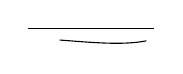
\begin{tikzpicture}
\draw (0,0)--(1.6,0);
\draw (.4,-.15).. controls (.8,-.18) and (1.2,-.22)..(1.5,-.16);
\end{tikzpicture}}

Soit $A$\inserted{$:(\unsure{\Delta}/X)^\circ\longrightarrow(\mathrm{Ab})$} un groupe sur $X$, considérons le complexe des cochaines sur $X$ à coeff. ds $A$
\[
C^{\unsure{n}}(X,A)\overset{\mathrm{dfn}}{=}
\prod_{\substack{\sigma\in\operatorname{Ob}\Delta_n/X\\=X_n}}A(\sigma)\quad,
\]
Les $C^n$ forment un groupe co $\frac12$ simplicial

\margin{59}

\scanpage{61}

\begin{center}- 152 -\end{center}
\begin{flushright}IX\end{flushright}

$\uline{\operatorname{Pic}}^{\unsure{o|0}}_{\widetilde C/k}$ est de ``rang réductif'' nul (i.e. son tore maximal est nul), de sorte que le tore maximal de $\uline{\operatorname{Pic}}^{\unsure{o|0}}_{C/k}$ est contenu dans
\[
N=\operatorname{Ker}(\uline{\operatorname{Pic}}_{C/k}
\longrightarrow\uline{\operatorname{Pic}}_{\widetilde C/k})\quad,
\]
donc est isomorphe canoniquement au tore maximal de ce dernier groupe. Or la structure de $N$ s'explicite aisément à l'aide de EGA IV 21.8.5 : on trouve que $N$ est canoniquement une extension d'un tore $T$ dont on va expliciter la description, par un groupe unipotent connexe $U$ (qui se dévisse de même, sur $k$, avec une suite de composition à quotients isomorphes au groupe additif $G_a$). D'ailleurs, si $T'$ est le tore maximal de $N$, alors $T'\cap U$ est à la fois unipotent et de type multiplicatif, donc nul (SGA 3 XVII 2.4), et l'image de $T'$ dans $T$ est identique à $T$ (SGA 3 XII 7.1 e)), de sorte que $T'\longrightarrow T$ est un isomorphisme. Donc $T$ est canoniquement isomorphe au tore maximal de $N$, donc de $\uline{\operatorname{Pic}}^{\unsure{o|0}}_{X/k}$.

C'est pour expliciter la structure de $N$ qu'il sera commode de supposer $k$ séparablement clos, de sorte que les composantes irréductibles $C_i$ de $C$ sont géométriquement irréductibles, et que les points non normaux de $C$ sont radiciels sur $k$. Ceci dit, soit $J$ l'ensemble des composantes irréductibles de $\widetilde C$, et pour tout $x\in C$, soit $J(x)$ l'ensemble des ``branches'' de $C$ passant par $x$ (i.e. des points de $\widetilde C$ au-dessus de $x$); soient enfin
\[
(12.3.1)\qquad R(x)=\mathbb Z^{J(x)}/\operatorname{Im}\mathbb Z\quad,
\]
où $\mathbb Z\longrightarrow\mathbb Z^{J(x)}$ est l'application diagonale, et
\[
(12.3.2)\qquad R=(\bigoplus_x R_x)/\operatorname{Im}\mathbb Z^J\quad,
\]

\margin{470}
\margin{470}
\margin{60}

\scanpage{62}

\diagram{\begin{tikzcd}
\Delta/X\arrow[r,"\text{fibration}"]&\Delta
\end{tikzcd}}

\deleted{
\diagram{\begin{tikzcd}
C\arrow[r]&B\\
C^\circ\arrow[d,"F"']&\\
\deleted{\unsure{(\mathrm{Ab})}}\inserted{\mathcal E}&
\end{tikzcd}}
\diagram{\begin{tikzcd}
C_b&i^*(x')\arrow[d]&b\arrow[d,"i"]\\
C_{b'}\arrow[u,"i^*"']&x'&b'
\end{tikzcd}}

\margin{(\unsure{adjoint})}
\diagram{\begin{tikzcd}[column sep=small]
(b\in B)\arrow[r,mapsto]&
{\displaystyle\unsure{\sum|\prod}_{x\in C_b}\unsure{F|R}(x)}
\arrow[r]&F(\unsure{i^*x'})\\
(b'\in B)\arrow[r,mapsto]&
{\displaystyle\sum_{x'\in C_{b'}}\unsure{F|R}(x')}
\arrow[u]\arrow[r]&
F(\deleted{\unsure{i^*}}\unsure{x'})\arrow[u]
\end{tikzcd}}
\deleted{$\unsure{\downarrow}$}

\diagram{\begin{tikzcd}[column sep=small]
(b\in B)\arrow[r,mapsto]&
{\displaystyle\prod_{x\in C_b}\unsure{F|R}(x)}
\arrow[d,"\unsure{?}"']\arrow[r]&
F(i^*x')\arrow[d]\\
(b'\in B)\arrow[r,mapsto]&
{\displaystyle\prod_{x'\in C_{b'}}F(x')}
\arrow[r]&F(x').
\end{tikzcd}}
\margin{$\unsure{f^*}$}
}

\margin{\unsure{?}}

Si
\diagram{\begin{tikzcd}
(\Delta/X)^\circ\arrow[r,"A_*"]&
\deleted{(\mathrm{Ab})}\inserted{\mathcal E\text{ (cat. avec sommes directes)}}
\end{tikzcd}}
est un faisceau sur $X$ (i.e. \deleted{\unsure{faisceau}}\inserted{syst.} de coeff. \uline{\unsure{contravariant}} \unsure{par r. à} un simplex variable sur $X$)
on lui associe
\[
C_*(X,A_*)=i_!(A):(\Delta\deleted{\unsure{/X}})^\circ\mathbin{-}\mathcal E
\]
(où $i:\widehat{\Delta/X}\longrightarrow\widehat{\Delta}$ est le morphisme d'induction des topos)

Si
\diagram{\begin{tikzcd}
\Delta/X\arrow[r,"A^*"]&
\deleted{(\mathrm{Ab})}\inserted{\mathcal E\text{ (cat. av. produits)}}
\end{tikzcd}}
est un ``cofaisceau'' sur $X$ (i.e. syst. de coeff. \uuline{cov.} \unsure{par r. à} un simplex variable de $X$) on lui associe $C^*(X,A^*)$
\[
\deleted{\unsure{co}}:(\Delta\deleted{\unsure{{}^\circ}})\mathbin{-}\mathcal E.
\]

On passe de l'un à l'autre en remplaçant $\mathcal E$ par $\mathcal E^\circ$; c'est compatible avec composition avec foncteur $\mathcal E\longrightarrow\mathcal E'$ qui commute aux sommes resp. produits.

\margin{61}

\scanpage{63}

\begin{center}- 149 -\end{center}
\begin{flushright}IX\end{flushright}

\uline{en associant à tout} $i\in I$ \uline{la section} $S_i$ \uline{de} $P$ \uline{sur} $S$ (\uline{nulle en} $\eta$) \uline{définie par le faisceau inversible} $\uline{O}_X(X_{\unsure{o|0}}^i)$ \uline{sur} $S$. (NB \uline{Comme les anneaux locaux de} $X$ \uline{sont factoriels en hypothèse}, \uline{les cycles} $X_{\unsure{o|0}}^i$ \uline{sont bien des diviseurs}, \uline{ce qui donne un sens à} $\uline{O}_X(X_i^{\unsure{o|0}})$ \uline{comme le faisceau inversible associé au diviseur en question} (EGA IV 21.2.8.1).) \uline{On a}
\[
(12.1.6)\qquad P^{\unsure{o|0}}\cap E=\text{\uline{section nulle de }}P\quad.
\]

c) \uline{Sous les conditions de} b), \uline{le quotient}
\[
(12.1.7)\qquad Q=P/E
\]
\uline{est représentable par un schéma en groupes lisse et séparé sur} $S$, \uline{et ce dernier est} néronien, \uline{i.e. satisfait la propriété universelle} (1.1.2) \uline{en termes de sa fibre spéciale}.

d) \uline{Sous les conditions de} c), \uline{supposons de plus que la fibre géométrique générique de} $X$ \uline{soit} intègre. \uline{Alors on a une suite exacte canonique}
\[
(12.1.8)\qquad
0\longrightarrow A\longrightarrow Q\xrightarrow{\deg}\mathbb Z_S\longrightarrow0\quad,
\]
\uline{où} $\deg$ \uline{est induit par l'homomorphisme} ``\uline{degré}'' $P\longrightarrow\mathbb Z_S$, \uline{et où} $A$ \uline{est un schéma en groupes lisse séparé et} de type fini \uline{sur} $S$, \uline{qui est également néronien i.e. qui est un modèle de Néron de}
\[
(12.1.9)\qquad A_\eta=P_\eta^{\unsure{o|0}}=\uline{\operatorname{Pic}}^{\unsure{o|0}}_{X_\eta/\eta}\quad.
\]
\uline{D'autre part, l'homomorphisme composé} $P^{\unsure{o|0}}\longrightarrow P\longrightarrow Q$ \uline{induit un isomorphisme}
\[
(12.1.10)\qquad P^{\unsure{o|0}}\xrightarrow{\sim}A^{\unsure{o|0}}\quad.
\]

\margin{467}
\margin{467}
\margin{62}

\scanpage{64}

\margin{(\unsure{$k$ anneau comm.})}
Mais si $F$\inserted{sur $X_*$}\inserted{(un $k$-Module)} est loc. constant, alors on vérifie facilement que
\[
C^*(X_*,F)\simeq
\Gamma\bigl(X_*,\underbrace{(C_*^*|X_*)}_{C_{X_*}^*}\otimes_{k_*}F\bigr)
\]
\margin{\figure{\begin{tikzpicture}
\node[draw,ellipse,align=left] {$\unsure{\text{NB on pose}}$\\$C_*^*=C_*^*k\quad\unsure{\text{pour abréger}}$};
\end{tikzpicture}}}

et on vérifie tout de suite que $C_{X_*}^*\otimes_{k_*}F$ est une résolution de $F$, laquelle est d'ailleurs \uline{flasque}. \deleted{\unsure{Donc}} (que $F$ soit loc. constant ou non, d'ailleurs). Donc, sans hypothèse de loc. constance sur $F$, $C^*(X_*,F)$ permet de calculer la coh. de $X_*$ à coeff. dans $F$ (i.e. \unsure{on a} un isom. can.
\margin{\figure{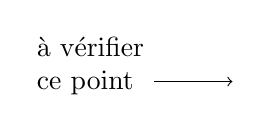
\begin{tikzpicture}
\node[align=left,anchor=east] at (0,0) {à vérifier\\ce point};
\draw[->] (0,-.2)--(1,-.2);
\end{tikzpicture}}}
\[
H^*\left(
\underbrace{C^*(X_*,F)}_{
\substack{\Vert\,\mathrm{dfn}\\\Gamma(X_*,C_{X_*}^*\otimes_kF)}
}
\right)\simeq H^*(X_*,F)
\]
\unsure{Isom.} \deleted{\unsure{compatible}} fonctoriel en $F$ (et même en $(X_*,F)\ldots$) et compatible avec les hom. cobords. De même pour le calcul de l'hypercohomologie de $X_*$ à coeff. ds un complexe de $k$-Modules $F^*$. En termes de catégories dérivées, on aura un isomorphisme de foncteurs triangulés
\[
R\Gamma(X_*,F^*)\simeq
\underbrace{C^*(X_*,F^*)}_{
\substack{\text{pour degré total}\\
\text{associé aux}\\
\text{deux degrés}\\
(\unsure{\text{proven. de }C\text{ et de}}\\F^*)}}
\]
\margin{\figure{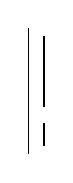
\begin{tikzpicture}
\draw (0,0)--(0,1.6);
\draw (.2,.6)--(.2,1.5);
\draw (.2,.1)--(.2,.4);
\end{tikzpicture}}}
\margin{63}

\scanpage{65}

Soit maintenant $A_*^{\unsure{\circ|*}}$ un \deleted{$k$-module} complexe de cochaines de $k$-modules $\frac12$ simpliciaux
\diagram{\begin{tikzcd}
0\arrow[r,dash]&A_*^0\arrow[r,dash]&A_*^1\arrow[r,dash]&A_*^2\arrow[r]&\cdots
\end{tikzcd}}
et proposons-nous de déterminer les homomorphismes de ce complexe dans
\diagram{\begin{tikzcd}
0\arrow[r,dash]&C_{*M}^0\arrow[r,dash]&C_{*M}^1\arrow[r,dash]&C_{*M}^2\arrow[r,dash]&\cdots,
\end{tikzcd}}
\inserted{où $M$ est un $k$-module donné}

Tout d'abord, les hom de degré $0$ (pas néc. \unsure{commutant} aux op. diff) sont les syst. d'hom
\diagram{\begin{tikzcd}
A_*^n\arrow[r,"u_n"]&C_{*M}^n
\end{tikzcd}}
i.e. les syst. d'hom de $k$-modules
\diagram{\begin{tikzcd}
A_n^n\arrow[r,"K_n"]&M
\end{tikzcd}}

\deleted{\unsure{On a :}}
L'hom composé
\[
d_C\circ u_n:
\]
\diagram{\begin{tikzcd}
A_*^n\arrow[r,dash]\arrow[rr,bend right=20]&C_{*M}^n\arrow[r]&C_{*M}^{n+1}
\end{tikzcd}}
correspond à l'hom composé
\diagram{\begin{tikzcd}[column sep=small]
A_{n+1}^n\arrow[rr,"K_n\partial_{n+1}"]\arrow[dr,"\partial_{n+1}"']&&M\\
&A_n^n\arrow[ur,"K_n"']&
\end{tikzcd}}

tandis que l'hom composé
\[
u_{n+1}\circ d_A:
\]
\diagram{\begin{tikzcd}
A_*^n\arrow[r]&A_*^{n+1}\arrow[r,dash]&C_{*M}^{n+1}
\end{tikzcd}}
correspond à l'hom composé
\diagram{\begin{tikzcd}[column sep=small]
A_{n+1}^n\arrow[rr]\arrow[dr,"d_A^n"']&&M\\
&\unsure{A_{n+1}^{n+1}}\arrow[ur,"K_{n+1}"']&
\end{tikzcd}}

\margin{64}

\scanpage{66}

et la condition que les $u_n$ définissent bien un hom de complexes est la ``condition de Stokes''
\[
K_n\partial_{n+1}=K_{n+1}d:
\]
\diagram{\begin{tikzcd}
A_{n+1}^n\arrow[r,"\partial_{n+1}"]\arrow[d,"d^n"']&
A_n^n\arrow[d,"K_n"]\\
A_{n+1}^{n+1}\arrow[r,"K_{n+1}"']&M
\end{tikzcd}}

Dans ces conditions, pour tt $X_*$\inserted{$\in\operatorname{Ob}\widehat{\Delta}$}, on a un hom. \unsure{can.} déduit de $u$
\diagram{\begin{tikzcd}
\Gamma(X_*,A_{X_*}^*)\arrow[r]&C^*(X_*,M_*)\arrow[d,equal]\\
&\Gamma(X_*,C_{\unsure{*}M}^*|X_*)
\end{tikzcd}}
qui représente l'hom dans la cat. dérivée
\[
\Gamma(X_*,A_{X_*}^*)\mathbin{-}\mathbb R\Gamma_{X_*}(M)
\]
associé à $u_*$. On aura alors \unsure{commutativité} dans
\diagram{\begin{tikzcd}[column sep=small]
\deleted{\mathbb R}\Gamma(X_*,A_{X_*}^*)\arrow[r]\arrow[d]&
C^*(X_*,M)=\Gamma(X_*,C_M^*|\unsure{X_*})\arrow[d,"\sim"]\\
\mathbb R\Gamma(X_*,A_{X_*}^*)\arrow[r]&
\mathbb R\Gamma(X_*,M)
\end{tikzcd}}

Si $A^*$ est une résolution de $M_*$, et $K_0:A_0^0\longrightarrow M$ induit l'identité sur $M\subset A_0^0$, alors la dernière flèche horizontale est aussi un iso, et

\margin{65}

\scanpage{67}

on peut considérer la flèche
\diagram{\begin{tikzcd}
\Gamma(X_*,A^*_{X_*}) \arrow[r] \arrow[d,equal] & \unsure{C|C^*}(X_*,M)\\
\operatorname{Hom}(X_*,A^*) &
\end{tikzcd}}
déduite du syst. de Stokes-DeRham $(K_n)$ comme une réalisation de l'hom. canonique
\diagram{\begin{tikzcd}
\Gamma(X_*,A^*_{X_*}) \arrow[r] & \mathbb R\Gamma(X_*,A^*_{\unsure{X_*|X}})\\
& \mathbb R\Gamma(X_*,M) \arrow[u,"\sim"]
\end{tikzcd}}

On voit que sous les conditions de la prop. 1, \unsure{il y}

\deleted{Supposons}

\uline{NB} L'hom
\[
\Gamma(X_*,A^n_{X_*})\xrightarrow{u^n}C^n(X_*,M)
\]
\margin{$\operatorname{Hom}(X_*,A_*^n)$}
associé à $K_n$ s'explicite ainsi: On considère, pour tt \unsure{élémt|élément} \deleted{\unsure{un}} $f:X_*\longrightarrow A_*^n$, l'application
\[
f_n:X_n\longrightarrow A_n^n
\]
et on prend
\[
u^n(f)=K_n\circ f_n\in\operatorname{App}(X_n,M)
\]

\figure{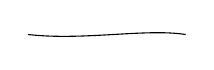
\begin{tikzpicture}\draw (0,0) .. controls (0.7,-.08) and (1.5,.08) .. (2,0);\end{tikzpicture}}

Supposons maintenant que $A_*^{\unsure{*|\circ}}$ soit un complexe \inserted{\unsure{de degrés $\geq 0$}} satisfaisant
\[
\begin{array}{ll}
\mathrm{a)}& A_n^i=0\quad\text{si }i>n\\
\mathrm{b)}& H^n(A_n^*)=0\quad\text{si }n\geq1\\
\mathrm{c)}& H^{n-1}(A_n^*)=0\quad\text{si }n\geq2
\end{array}
\]
\margin{(\unsure{il suffit|i.e. suffit} $A_n^n=Z_n^n$ i.e. $d(A_n^n)=0$ si $n\geq1$)}
Alors on sait qu'un syst. $K_n:A_n^n\longrightarrow M$ satisfaisant la condition de Stokes

\figure{\begin{tikzpicture}\draw (0,0)--(0,1.25);\draw (.16,.2)--(.16,1.15);\end{tikzpicture}}
\margin{66}

\scanpage{68}

est déterminé par la connaissance de
\[
K_0:A_0^0=A_0\longrightarrow M
\]
et $K_0$ \unsure{quelconque}, un $(K_n)$ \unsure{'|$\exists$} ssi
\[
K_0\bigl(\partial_1(\operatorname{Ker}(A_1^0\xrightarrow{d}A_1^1))\bigr)=0
\]
(donc il y a un syst. d'intégrale de Stokes-DeRham ``universel'' à valeurs dans
\[
A_0/\partial_1(\operatorname{Ker}(A_1^0\xrightarrow{d}A_1^1)),
\]
le cas le plus intéressant est celui où
\[
\partial_1(\operatorname{Ker}(A_1^0\overset{d}{\text{---}}A_1^1))=0,
\]
donc où le \unsure{choix universel|domaine universel} est pour $M=A_0$, ce qui sera le cas en particulier si on a
\[
\mathrm{c}')\quad H^0(A_1^*)\xleftrightarrow{\sim}\varepsilon^*(A_0^0)
\qquad(\text{où }\varepsilon:\Delta_1\longrightarrow\Delta_0\ldots)
\]
(ce qui est une variante de c) pour $n=1$).

\margin{ou $H^0(A_1^*)=\varepsilon^*(Z_0^0)$ \unsure{dans le cas où l'on présume a), en général}}
\figure{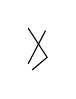
\begin{tikzpicture}\draw (0,.45)--(.24,.08)--(.05,-.08);\draw (0,0)--(.22,.42);\end{tikzpicture}}

Sous ces conditions, on sait donc qu'il existe un \uline{unique} hom de complexes de modules $1/2$ simpliciaux
\[
A_*^*\longrightarrow C_{*M}^*.
\]
qui sur $A_0^0=A_0$ coïncide avec
\[
K_0:A_0^0\longrightarrow \unsure{C|R}_{0M}^0=M
\]
(donc l'identité; le \unsure{cas|syst.} prototype).

On peut noter qu'en fait cet hom est même à valeurs dans $C_{*M}^{*!}$ (les cochaines non dégénérées), i.e. on a en fait
\[
A_*^*\longrightarrow C_{*M}^{*!}\simeq
\Lambda^{*+1}\unsure{\Phi|Q}_{*k}\otimes_k M
\]
en se rappelant que
\[
C_{*M}^{n!}=
\bigcap_{\unsure{\sigma:\Delta_n\twoheadrightarrow\Delta_m,\ m<n}}
\operatorname{Ker}(C_{*M}^{n}\xrightarrow{\sigma^*}C_{*M}^{m})
\]
\margin{67}

\scanpage{69}

donc
\[
\operatorname{Hom}(A_*^n,C_{*M}^{n!})
=\{A_*^n\xrightarrow{\unsure{f^n|f^*}}C_{*M}^n\mid
\sigma^*f=0\ \forall\sigma:\Delta_n\longrightarrow\Delta_m\
\unsure{\text{surj.}}\ m<n\}
\]
\margin{\diagram{\begin{tikzcd}
A_*^n \arrow[r,dash,"f^n"] \arrow[d,"\sigma_A^*"'] & C_*^n) \arrow[d,"\sigma_C^*"]\\
A_*^m \arrow[r] & C_*^m
\end{tikzcd}}}
Or $A_*^n\text{---}C_*^n$ est donné par \deleted{\unsure{$A$}}
\[
A_n^n\xrightarrow{\unsure{K_n|k_n}}M
\]
son composé $A_*^n\text{---}C_*^n\text{---}C_*^m$ est donné par le
\[
A_m^n\longrightarrow M
\]
qui n'est autre que le composé
\[
A_m^n\xrightarrow{\sigma^*}A_n^n\xrightarrow{\unsure{K_n|k_n}}M
\]
et la condition \deleted{\unsure{$f(A_*^n)$}} on a donc
\[
f^n(A_*^n)\subset C_*^n
\Longleftrightarrow
\left|\begin{array}{l}
\unsure{K_n|k_n}\circ\sigma^*=0\\
\forall\sigma:\Delta_n\longrightarrow\Delta_m,\quad m<n
\end{array}\right.
\]
(il suffit de le vérifier qd $\sigma$ est un op de dégénérescence); or cette condition est tjs satisfaite si $A_m^n=0$ si $m<n$, ce qu'on a supposé dans a).

\uline{Ex} Soit $S$ un anneau à \unsure{idéal} $J$ à p.d., $t\in J$, considérons alors cet anneau différentiel $1/2$ simplicial à p.d.
\[
A_*^*=(\Gamma^*(\unsure{\Phi|Q}_{*S})\otimes_S\Lambda^*\Psi_{*S})/(T-t)_{\mathrm{pd}},
\]
c'est une \uline{résolution} de $S$, et $A_j^i=0$ si $i>j$, donc on a un syst. d'\unsure{intégrales|intégrale} de Stokes-DeRham à valeurs dans $S$, donc
\diagram{\begin{tikzcd}
A_*^* \arrow[r,"\sim"]&
\left(\Gamma^*(\unsure{\Phi|Q}_{*S})\otimes_S
\Lambda^*\Psi_{*S}/(T-t)_{\mathrm{pd}}\right)
\arrow[dr] &\\
&&\Lambda^{*+1}\unsure{\Phi|Q}_{*S}
\end{tikzcd}}
dont il faudrait étudier les propriétés \unsure{multiplicatives}.
\margin{\deleted{\unsure{p.d.}}}
\margin{68}

\scanpage{70}

\textcircled{1}\quad
$k_*\xrightarrow{\varepsilon_*}A_*^*$,
$K_*=(K_n)_{n\geq0}$,
$K_n:A_n^n\text{---}k$, satisf.
$\left\{\begin{array}{l}\text{Stokes}\\ K_0\varepsilon_0=\mathrm{id}\end{array}\right.$

\textcircled{2}\quad Sur un \deleted{\unsure{topos}} espace topologique $X$,
faisceau différentiel \inserted{de $S$-modules}
\deleted{\unsure{$E$}} $\Omega^*$ qui est une \uline{résolution} de $k_X$
(p.ex. complexe de DR sur $X$ variété $C^\infty$, $k=\mathbb R=S$)

\textcircled{3}\quad Un sous-ensemble $1/2$ simplicial $S(X)'$ du complexe singulier de $X$, tel que
$S(X)'\text{---}S(X)$ \deleted{\unsure{soit}} induise un isom sur les \unsure{gr.} d'homologie entière
(p.ex. $X$ est une variété $C^\infty$ et $S(X)'$ est formé des simplexes $C^\infty$)
\inserted{\unsure{et si on remplace} $X$ \unsure{par un ouvert}
(d'une base) et qu'on \unsure{prend dans} $S(X)$ et $S(X)'$
\unsure{les sous-complexes des simplexes} de \uline{support $\subset U$}!
\deleted{\unsure{$J$}}}

\margin{donc, si on regarde le \uline{faisceau} \deleted{\unsure{de}}
de \unsure{coch.} sing. $S^*_{X,k}$ sur $X$, et de même
$S_{X,k}^{*'}$, $S_{X,k}^{*'}$ est comme $S_{X,k}^*$ une rés. de $k$}
\figure{\begin{tikzpicture}\draw[->] (4,0) .. controls (3,.7) and (1,.6) .. (0,.6);\end{tikzpicture}}

\textcircled{4}\quad $\forall\sigma\in S(X)'$, est
\deleted{\unsure{donné un morphisme}}
\inserted{\unsure{un hom. de}} $k$-augm.
\[
\sigma^*:\underset{\substack{U\text{ ouvert de }X\\ U\supset\operatorname{supp}\sigma}}{\varinjlim}
\Omega^*(U)\longrightarrow A_n^*
\qquad(n=\dim\sigma)
\]

On suppose que si $\alpha:\Delta_m\longrightarrow\Delta_n$,
$\sigma\in S'(X)_n$,
\deleted{\unsure{$\sigma:|\Delta_n|\longrightarrow X$}}
on a commutativité dans
\diagram{\begin{tikzcd}
\underset{U\supset\operatorname{supp}\sigma}{\varinjlim}\Omega^*(U)
\arrow[r]\arrow[d,"\text{restriction}"'] & A_n^*\arrow[d,"\unsure{\sigma_A^*|\alpha_A^*}"]\\
\underset{V\supset\operatorname{supp}\alpha^*(\sigma)}{\varinjlim}\Omega^*(V)
\arrow[r] & A_m^*
\end{tikzcd}}
\margin{\uline{NB} $\operatorname{supp}\alpha^*(\sigma)\subset\operatorname{supp}\sigma$}

[\uline{NB} On peut dire que
\[
\sigma\longmapsto\underset{U\supset\operatorname{supp}\sigma}{\varinjlim}\Omega^*(U)
\]
forme un \deleted{\unsure{faisceau}} objet semi-simplicial
$\Omega^*_{S(X)'}$ (en fait un complexe de $S$-modules
$k$-augmenté) sur $S(X)'=\mathcal X$,
et on se donne un hom de celui-ci dans le complexe \unsure{analogue}
$A^*_{\mathcal X}$ sur $\mathcal X=S(X)'$ défini par
$A_*^*\times\mathcal X$.

\margin{\diagram{\begin{tikzcd}
\Delta_n\arrow[dr,"\sigma"'] & \Delta_m\arrow[l,"\alpha"']\arrow[d,"\alpha^*(\sigma)=\sigma\circ\alpha"]\\
& S(X)'=\mathcal X
\end{tikzcd}}}

\uline{NB} finalement \textcircled{1} $(A_*^*,k_*,K_*)$
\inserted{et (4)} ne servent que pour pouvoir définir
\[
\unsure{\varphi:|\leftrightarrow}\quad\Omega^*\longrightarrow S_X^{*'}
\quad\unsure{\text{comp. coch. augm.}}
\]
\margin{69}

\scanpage{71}
\margin{- 140 -}
\margin{IX}

où par définition $({}_n A_K)^f=({}_n A^o)_K^f$ désigne le r.ème composant $(n=\ell^{r+1})$ du pro-groupe de Barsotti-Tate $T_\ell(A_K)^f$. La première des relations (5.5.8) nous fournit alors un isomorphisme canonique
\[
(11.6.7)\qquad {}_n\Psi_K\simeq\underline M_{nK}
\qquad\text{où }\underline M_n\overset{\mathrm{dfn}}=
\underline M\otimes_{\mathbb Z}(\mathbb Z/n\mathbb Z).
\]
En fait, on a :

\uline{Lemme} 11.6.8. \uline{Le schéma en groupes} $ {}_n\Psi$ (11.6.6) \uline{sur} $S$ \uline{est étale sur} $S$, \uline{et l'isomorphisme} (11.6.7) \uline{se prolonge de façon unique en un morphisme}
\[
(11.6.8.1)\qquad {}_n\Psi\lhook\joinrel\longrightarrow\underline M_n
\]
\uline{qui est une immersion ouverte}.

Pour voir que $ {}_n\Psi$ est étale, il reste à vérifier en vertu de (11.6.7) qu'il l'est en les points de sa fibre spéciale, ou encore que cette dernière est étale, ce qui est trivial, la fibre en question étant
$ {}_n A_o/{}_n A_o^o\subset A_o/A_o^o=\Phi_o$.
Il s'ensuit que $ {}_n\Psi$ est un schéma normal, et comme $\underline M_n$ est fini sur $S$, l'existence d'un prolongement (11.6.8.1) en résulte aussitôt. C'est un morphisme de schémas en groupes étales sur $S$, donc son noyau est un groupe étale sur $S$, et comme $ {}_n\Psi$ donc ce noyau est séparé, et sa fibre générique est le groupe unité par (11.6.7), c'est le groupe unité (3.1.3). Donc (11.6.8.1) est un monomorphisme étale, donc une immersion ouverte (EGA IV 17.9.1), ce qui prouve le lemme.

Posons maintenant
\[
(11.6.9)\qquad {}_n\Phi=({}_n A)^f/({}_n A^o)^f\subset{}_n\Psi,
\]
de sorte que $ {}_n\Phi$ est un sous-schéma fini ouvert de $ {}_n\Psi$, puisque $({}_n A)^f$

\margin{458}
\margin{458}
\margin{70}

\scanpage{72}

\deleted{\diagram{\begin{tikzcd}[column sep=small]
\deleted{C^*(X,\Omega^*)}\arrow[r]&
\deleted{\mathbb R^*\Gamma(X,\Omega^*)}&
\mathbb R^*\Gamma(X,k)\arrow[l,"\varepsilon_{\Omega^*}"']\arrow[r,"\sim","{\varepsilon_{S_X^*}}"']\arrow[d,"\sim"']\arrow[dr,dashed,"\varepsilon_{S_X^{\prime *}}"]&
\mathbb R^*\Gamma(X,S_X^*)\arrow[d,"\sim"]&
\Gamma(X,S^*_{X,\unsure{k}})=C^*(S(X)_*,k)\arrow[l,"\sim"']\arrow[d,"\sim"]\\
&&\mathbb R^*\Gamma(X,\Omega^*)\arrow[r,"\sim"]&
\mathbb R^*\Gamma(X,S_X^{\prime *})&
\Gamma(X,S_X^{\prime *})=C^*(S(X)'_*,k)\arrow[l,"\sim"']\\
&&C^*(X,\Omega^*)\arrow[u]&&
\end{tikzcd}}}
\margin{($S_X^*$ \unsure{homot$^t$ fin}; \unsure{système paracompact})}

\uline{NB} \unsure{les hyp.} (4) \unsure{jointes|jointe} avec
$\unsure{K_*|k_*}$ définit un hom
$\Omega^*\longrightarrow S_X^{\prime *}$ compatible avec les augmentations,
d'où carré comm.
\diagram{\begin{tikzcd}
\Omega^*\arrow[r,"\unsure{\text{par }K}"{ellipse,draw}]&S_X^{\prime *}\\
k\arrow[u]\arrow[r,dash]&S_X^*\arrow[u]
\end{tikzcd}}
\deleted{\unsure{(isom.}}
(d'isom dans $D(X,S)$) donnant lieu à un cube commutatif

\diagram{\begin{tikzcd}[column sep=small,row sep=large]
C^*(X,\Omega^*)\arrow[rr]\arrow[dd,"\unsure{q}"]\arrow[dr,phantom,"\deleted{\unsure{\searrow}}"]&&
C^*(X,S_X^{\prime *})\overset{\mathrm{dfn}}=C(S'_X,k)\arrow[dd,"\sim"]&\\
&[C(X,k)]\arrow[ul,dashed]\arrow[rr,dashed]\arrow[dd,dashed]&&
C^*(X,S_X^*)=C(S_X,k)\arrow[ul,"\sim\ \text{pr. sur }S'_X"']\arrow[dd,"\sim\ (\text{Cartan, }S_X^*\text{ est }\unsure{\text{``homot}^t\text{ fin''}})"]\\
\mathbb R^*\Gamma(X,\Omega^*)\arrow[rr,"\sim"]&&\mathbb R^*\Gamma(X,S_X^{\prime *})&\\
&\mathbb R^*\Gamma(X,k)\arrow[ul,"\sim"]&&
\mathbb R^*\Gamma(X,S_X^*)\arrow[ul,"\sim"]\arrow[ll,"\unsure{\sim}"]
\end{tikzcd}}

\margin{\deleted{$\longleftarrow\mathbb R^*\Gamma(X,S^*_{X,\unsure{k}})$}}

Le bas du cube est formé d'isom, car transformé par $\mathbb R^*\Gamma$ d'un carré d'iso dans une cat. dérivée; la face \unsure{droite} est formée d'iso, car on le sait déjà pour deux arêtes, donc aussi pour la quatrième qui reste.
\margin{71}

\scanpage{73}
\margin{- 139 -}
\margin{IX}

définir l'isomorphisme canonique (11.6.2).

Ecrivant $M_\ell\otimes D_\ell$ (resp. $\check M_\ell\otimes D_\ell$) comme limite inductive des $M_n$ (resp. des $\check M'_n$), où $n$ parcourt les puissances de $\ell$, il revient au même de définir (11.6.2), où des isomorphismes canoniques
\[
(11.6.4)\qquad {}_n\Phi_o\simeq\operatorname{Ker}
\{\widetilde u_n:M_n\longrightarrow\check M'_n),\quad n=\ell^{r+1},
\]
comptatibles avec les morphismes de transition évidents, pour $n$ variable
(où $\widetilde u_n$ désigne maintenant, par abus de notations, l'homomorphisme déduit de $\widetilde u_\ell:M_\ell\longrightarrow\check M'_\ell$ par réduction mod. $n$).

Pour ceci, considérons le schéma en groupes $ {}_n A$ sur $S$, qui est plat et quasi-fini sur $S$ (2.2.1), grâce à l'hypothèse de réduction semi-stable. On a une filtration canonique
\[
(11.6.5)\qquad {}_n A\supset({}_n A^o)^f\supset({}_n A^o)^t\supset0,
\]
où l'exposant $f$ (resp. l'exposant $t$) désigne la ``partie fixe'' (2.2.3) (resp. la ``partie torique'' (5.1)) du schéma en groupe qu'il affecte ; pour la définition de la partie torique dans 5.1, on notera qu'on avait supposé $S$ complet, ce qui est loisible ici (11.0). (On a d'ailleurs vu dans 6.1 que la construction se généralise au cas $S$ hensélien, si on y tient \ldots) Soit
\[
(11.6.6)\qquad {}_n\Psi={}_n A/({}_n A^o)^f,
\]
c'est un schéma en groupes plat, séparé et quasi-fini sur $S$ (SGA 3 $\mathrm{VI}_A$ 3.2 et $\mathrm{VI}_B$ 9.2) de fibre générique
\[
{}_n\Psi_K=({}_n A_K)/({}_n A_K)^f,
\]

\margin{\figure{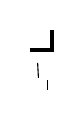
\begin{tikzpicture}
\draw[line width=1.5pt] (0,.4)--(.28,.4)--(.28,.66);
\draw (.1,.24)--(.11,.05);\draw (.22,.02)--(.22,-.1);
\end{tikzpicture}}}
\margin{\unsure{457}}
\margin{\unsure{13|B}}
\margin{457}
\margin{72}

\scanpage{74}
On travaille dans le topos ss $(SS)=\widehat{\Delta}$, avec $k$ anneau comm.

\[
\begin{aligned}
\Phi_*&=\Phi_*k=i_{0*}(k)\\
&=\Phi_{*\mathbb Z}\otimes_{\mathbb Z}k\\
&=\Phi_{*\mathbb Z}\otimes_{\mathbb Z_*}k_* .
\end{aligned}
\]
\deleted{\unsure{J}} on le considère comme faisceau de $k$-modules, (pas comme faisceau d'anneaux) muni d'une section $T$
\[
\left\{\begin{aligned}
T&\in\Gamma(SS,\Phi_*k)\inserted{[=\Gamma(SS,C_*^{10})]}\\
k_*&\hookrightarrow\Phi_*k
\end{aligned}\right.
\quad\text{définissant un \uline{\unsure{régulier}}}.
\]
On a la $k$-Algèbre bigraduée \deleted{\unsure{gr.}} différentielle à p.d.
\[
C_{*k}^{**}\unsure{:=|=}C_{*k}^{**}
=\deleted{\unsure{\Lambda}}\inserted{\Gamma_k^*}\Phi_*\otimes_k\Lambda^*\Phi_*
\]
\margin{(diff. de bidegré $-1,+1$ $\cdots$) \deleted{\unsure{alg.}} alg. \unsure{alternée} pour degré ext,}
qui est une résolution de $k$. De façon précise,
$C_{*k}^{00}=k_*$, et en degré \unsure{total|tot.} donné $n>0$,
on trouve une suite exacte
\[
\begin{gathered}
0-\Gamma^n\Phi^*-\Gamma^{n-1}\Phi^*\otimes\Lambda^1\Phi^*
-\Gamma^{n-2}\Phi^*\otimes\Lambda^2\Phi^*\longrightarrow\\
\cdots\longrightarrow\Phi^*\otimes\Lambda^{n-1}\Phi^*
\longrightarrow\Lambda^n\Phi^*\longrightarrow0\longrightarrow0\cdots
\end{gathered}
\]
dont les termes sont donc flasques.
\margin{Notons $\bar\Phi_*\unsure{\mathrel{\vdash}|:=}\Lambda^1\Phi_*$
et $\bar x$ pour \deleted{\unsure{de}} l'élément \deleted{\unsure{de}} \unsure{de} $\bar\Phi_*$
\unsure{correspondant à} \deleted{\unsure{l'élément}} $x$ de $\Phi_*$.}

On considère $\underset{\Vert\,\bar T}{dT}\in
\Gamma(SS,\deleted{\unsure{\Phi_*}}C_*^{01})\simeq\Gamma(SS,\bar\Phi_*)$
et l'homomorphisme
\[
\bar T_{\wedge}:C_*^{**}\longrightarrow C_k^{**},
\]
on voit qu'il est de bidegré $(0,1)$, \inserted{de carré nul, $\operatorname{Im}(\bar T_\wedge)=\operatorname{Ker}(\bar T_\wedge)$}
\inserted{anti}commutant à $d$
\[
\bigl(d(\bar T\cdot x)=\underset{\Vert\,0}{d\bar T}\cdot x-\bar T\,dx=-\bar T\,dx\bigr),
\]
est injectif sur $C^{*0}$. On pose
\[
\begin{aligned}
DR_{*k}^{pq}=DR_*^{pq}
&=\operatorname{Ker}(C_*^{p,q+1}\xrightarrow{\bar T_\wedge}C_*^{p,q+2})\\
&=\operatorname{Ker}(\Gamma^p\Phi_*\otimes\Lambda^{q+1}\Phi_*-\Gamma^p\Phi_*\otimes\Lambda^{q+2}\Phi_*)\\
&\simeq\deleted{\unsure{\operatorname{Ker}(}}\Gamma^p\Phi_*\otimes
\underbrace{\operatorname{Ker}(\Lambda^{q+1}\Phi_*-\Lambda^{q+2}\Phi_*)}_{\Lambda^q\Psi_*},
\qquad\Psi_*=\Phi_*/k_*\\
&\simeq\Gamma^p\Phi_*\otimes\Lambda^q\Psi_*,
\end{aligned}
\]
$DR_*^{**}=(DR_*^{pq})_{(p,q)\in\mathbb Z\times\mathbb Z}$, avec la bigraduation et la différentielle \inserted{(au signe près)} induites par $C_*^{**}$,
\deleted{\unsure{sauf que}} (mais avec décalage d'une unité pour le degré ext), et une structure multiplicative \deleted{qui} et à p.d. qui sont compatibles
\margin{73}

\scanpage{75}
par la propriété que l'hom épi
\[
u\unsure{=|\ne}\bar T_\wedge:\quad C_*^{**}\xrightarrow{u}DR_*^{**}\overset{i}{\subset}C_*^{**}
\]
soit compatible à ces structures (est faux; \unsure{à} \uline{\unsure{tuer|lier}} ces structures).
On aura aussi
\[
\deleted{\unsure{i(u(x)u(y))=}}\qquad
\left\{\begin{aligned}
i(xu(y))&=i(x)y\\
i(u(y)x)&=yi(x)
\end{aligned}\right.
\qquad i(x)i(y)=0 .
\]
Notons qu'on a la suite exacte
\diagram{\begin{tikzcd}[column sep=large]
0\arrow[r]&DR_*^{p,q}\arrow[r,dash,"i"]&
C_*^{p,q+1}\arrow[r,"(\bar T_\wedge)=u"]&
DR_*^{p,q+1}\arrow[r]\arrow[d,phantom,"\cap" description]&0\\
&&&C_*^{p,q+2}&
\end{tikzcd}}
et que le noyau $DR_*^{\unsure{pq|qp}}$ est flasque si $p\geq0$ --
donc si $X_*\in\operatorname{Ob}SS$, $\operatorname{Hom}(X_*,-)$ dans cette suite exacte donne encore une suite exacte
(i.e. \deleted{\unsure{injectif}} $C^{p,i}(X_*)\overset{\bar T}{-}DR^{p,i}(X_*)$ est surjectif).

Passons donc à $\operatorname{Hom}(X_*,-)$.
\[
C^{**}=C_*^{**}(X_*)=C^{**}(X_*,k)
\]
est une $k$-Algèbre bigraduée différentielle à p.d., avec \unsure{élémt|élément} marqué $T\in C^{1,0}$
\[
(A)\quad
\left\{\begin{aligned}
C^{00}\inserted{=H^{00}}&\simeq k^{\pi_0(X_*)}\deleted{\unsure{k}}(=k\text{ si }X_*\text{ connexe}),\\
H^{pq}(C^{**})&=0\quad\text{si }pq\ne0,\quad -
\end{aligned}\right.
\]
Posons $\bar T=dT\in C^{0,1}$, on a de plus
\[
(B)\quad\left\{\begin{gathered}
0\longrightarrow C^{p,0}\xrightarrow{\bar T_\wedge}C^{p,\unsure{1|q+1}}
\xrightarrow{\bar T_\wedge}C^{p,2}\longrightarrow\cdots
\longrightarrow C^{p,q}\overset{\bar T_\wedge}{-}C^{p,q+1}-\\
\text{est une suite exacte si }p>0
\end{gathered}\right.
\]
tandis que, pour $p=0$, comme
\[
\deleted{\unsure{\Phi}}\quad
0-\underset{\Vert\,k_*}{\Lambda^0\Phi_*}
\xrightarrow{\bar T_\wedge}\Lambda^1\Phi_*
\overset{\bar T_\wedge}{-}\Lambda^2\Phi_*-
\]
est une suite exacte fournissant une résolution flasque de $k_*$, on trouve
\[
\begin{gathered}
H^{\unsure{n}}\bigl(0-C^{0,0}\xrightarrow{\bar T_\bullet}C^{0,1}
-\cdots\longrightarrow C^{0,q}\overset{\bar T_\bullet}{-}C^{0,q+1}-\cdots\bigr)\\
\simeq\begin{cases}
0&\text{si }n\leq1\\
H^{n-1}(X_*,k)&\text{si }n\geq2
\end{cases}
\end{gathered}
\]
\margin{74}

\scanpage{76}
Posant
\[
DR^{pq}=DR^{pq}(X_*)=\operatorname{Ker}(C^{p,q+1}\xrightarrow{\bar T_\bullet}C^{p,q+2}),
\qquad DR^{**}=(DR^{pq})_{p,q\in\unsure{\mathbb Z|\mathbb Z^2}},
\]
on aura donc
\diagram{\begin{tikzcd}[column sep=large]
C^{p,q}\arrow[r,"\bar T_\bullet=u","\text{épi si }p\ne0"']&
DR^{pq}\arrow[d,phantom,"\cap" description]\\
&C^{p,q+1}
\end{tikzcd}}
d'où
\diagram{\begin{tikzcd}
C^{**}\arrow[r,dash,"u"]&DR^{**}\arrow[d,phantom,"\cap\,i" description]&\deleted{\unsure{u}}\\
&C^{**}&
\end{tikzcd}}
\margin{\figure{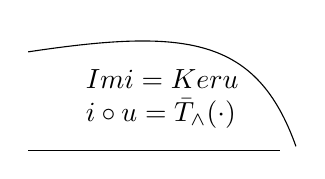
\begin{tikzpicture}
\node[align=left] at (0,0) {$\operatorname{Im}i=\operatorname{Ker}u$\\$i\circ u=\bar T_\wedge(\cdot)$};
\draw (-1.7,.6) .. controls (.3,.9) and (1.2,.8) .. (1.7,-.6);
\draw (-1.7,-.65)--(1.5,-.65);
\end{tikzpicture}}
$(C)\quad i(x)\cdot i(y)=0$}
\margin{(il est évident que $i(DR)\uline{i(uDR)=0}$ donc
$i(DR^{p,q})i(DR^{p',q'})=0$ si \unsure{$p$ ou $p'$}$\ne0$)}
\inserted{et} on aura sur $DR^{**}$ une structure bigraduée différentielle à p.d.
\deleted{telle que}
\inserted{\unsure{comm. gr.}, aux axiomes usuels (\unsure{alternée etc})}
\[
u:C^{**}\longrightarrow\unsure{D^{**}|DR^{**}}
\]
soit compatible avec ces structures
\inserted{et $\left\{\begin{aligned}i(xu(y))&=i(x)y\\i(u(y)x)&=yi(x)\end{aligned}\right.$}.
Ces structures sur $DR^{**}$ sont presque déterminées par ces propriétés, plus celle que l'inclusion
$DR^{**}\subset C^{**}$ est de bidegré $0,1$ et \inserted{anti}commutant à la différentielle -- à la détermination près des produits $xy$ \deleted{$\unsure{x^n}$} et des puissances divisées
$x^{(i)}$ $(i\geq2)$ quand $x,y$ \deleted{\unsure{sont}} de \unsure{degré complémentaire 0},
\margin{\unsure{donc (C) si que|donc (C) i.e.}
\figure{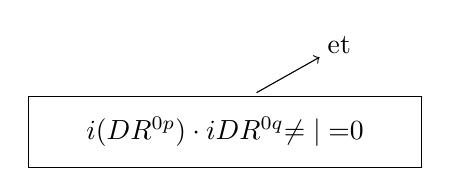
\begin{tikzpicture}
\node at (0,0) {$i(DR^{0p})\cdot iDR^{0q}\unsure{\ne|=}0$};
\draw (-2.5,-.45)--(2.5,-.45)--(2.5,.45)--(-2.5,.45)--cycle;
\draw[->] (.4,.5)--(1.2,.95);
\node at (1.45,1.1) {et};
\end{tikzpicture}}}

(auquel cas on ne peut pas néc. les écrire sous la forme $u(x')$
\inserted{\deleted{\unsure{et}} ou $u(y')$} ($x'$ dans $C^{**}$)).

(\uline{NB} Il est visible que sur \deleted{\unsure{DR}} \unsure{$DR\times DR$}, pour définir
\inserted{\uline{de faç. unique}} une multiplication
\deleted{\unsure{satisfaisant}}
\inserted{\unsure{coïncidant sur} $(\operatorname{Im}u)\times DR$ et $DR\times\operatorname{Im}u$}
\[
u(x,y)=u(x)u(y),\qquad i(xu(y))=i(x)y,\qquad i(u(y)x)=yi(x)
\]
(\deleted{\unsure{car}} la première relation équivaut, en appliquant $i$, à
$\bar T_\bullet(xy)=i(ux\cdot uy)$, d'où en appliquant la deuxième
\[
\bar T\cdot(xy)=(\bar T\cdot x)y
\]
donc il suffit de vérifier l'existence et l'unicité de
$\operatorname{Im}u\times DR-DR$ et $DR\times\operatorname{Im}u-DR$
satisfaisant les rel. 2 et 3. Or pour la $2^{\text{ème}}$, il suffit de montrer que

a) $i(x)y\inserted{=xy}\in\deleted{\operatorname{Ker}\unsure{\bar T}}DR=\operatorname{Ker}(\bar T_\wedge)$

car $\bar T(xy)=(\bar T x)y=0$ car $\bar T x=0$ puisque $x\in DR$

b) $i(x)y\inserted{=xy}$ ne dépend que de $x\in DR$ et de $uy\in\unsure{BR|DR}$,

car si $uy)=0$ i.e. $\bar T y=0$, i.e. $y\in DR$, on a
$xy=0$ -- Idem pour 3.
\margin{75}

\scanpage{77}
De \unsure{$=$|m.}, on a sur $u(C^{**+})\subset DR^{**+}$ des op.
``puiss. div.'' \inserted{uniques} données par la condition
\[
u(x)^{(i)}=u(x^{(i)})
\]
car il suffit de prouver que si $x'$ est tel que
$ux=ux'$, i.e. $x'=x+y$, $\bar T\cdot y=0$, alors
\inserted{$u(x'^{(i)})=u(x^{(i)})$, i.e. $\bar T_\wedge x'^{(i)}=\bar T x^{(i)}$}
\[
x'^{(i)}=x^{(i)}+x^{(i-1)}y+x^{(i-2)}y^{(2)}-+y^{(i)}
\]
il suffit de prouver que $\bar T y^{(i)}=0$ pour $i\geq1$,
ce qui résulte du fait \deleted{\unsure{évident}}\inserted{que}
\[
\text{\textcircled{D}}\qquad
\inserted{\text{sur}}\quad
\underset{\Vert\,\operatorname{Ker}(\bar T_\wedge(\cdot))}{DR^{**+}}\subset C^{**}.
\quad\deleted{\text{est stable par}}
\quad\begin{gathered}
\text{les puiss. div. (dans }C^{**}\text{)}\\
y^{(i)}\ (i\geq2)\ \text{\uline{sont} nulles}
\end{gathered}
\]
\deleted{i.e. si $y\in C^{**+}$, $\bar T\cdot y=0\longrightarrow\bar T\cdot y^{(i)}=0\quad\forall i\geq1$,}

(Ceci sera donc visible sur la construction pour $DR_*^{**}\subset C_*^{**}$,
où loc. $y$ est de la forme $\bar Tz$, donc
$\deleted{\unsure{\bar T_\wedge}}y^{(i)}=\bar T^i z^{(i)}$,
qui est donc nul si $i\geq2$.)

\deleted{(\unsure{NB|E}) $\unsure{DR^{**+}}\bar T(\unsure{x\in DR^{p,0}\subset C^{p,1}})\unsure{=0}$}

Ainsi, les seules données supplémentaires sur $C^{**}$ pour
\deleted{définir}\inserted{décrire} les structures habituelles sur $DR^{**}$ sont
\[
(E)\quad\left\{\begin{aligned}
&\text{``multiplication''}\quad
\unsure{DR}^{0,p\deleted{\unsure{+1}}}\times
\unsure{DR}^{0,q\deleted{\unsure{+1}}}\longrightarrow
\unsure{DR}^{0,p+q\deleted{\unsure{+1}}}
\quad(p,q\geq1)\\
&\text{``puiss. divisées''}\quad
\unsure{DR}^{0,p}\xrightarrow{\gamma^i}
\unsure{DR}^{0,pi\deleted{\unsure{+1}}}
\quad(i\geq2)
\end{aligned}\right.
\]
\margin{(\uline{\unsure{données}})}
\deleted{(\uline{NB} \unsure{sur}
$Z^{0,1}\times Z^{0,q+1}-$ pour $p$ ou $q=1$,
$-\unsure{Z^{0,p+q+1}}$ puisque $Z^{0,1}$ est engendré par}
\figure{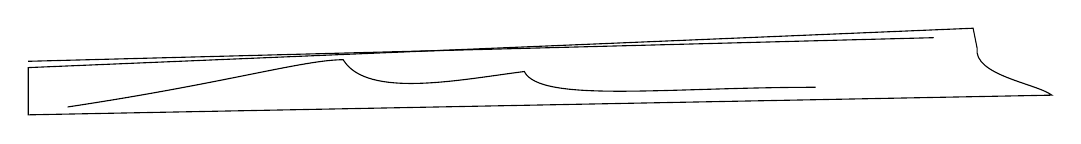
\begin{tikzpicture}
\draw (0,0)--(12,.5)--(12.05,.25) .. controls (12,-.1) and (12.8,-.2) .. (13,-.35)
--(0,-.6)--cycle;
\draw (0,.08)--(11.5,.38);
\draw (.5,-.5)..controls(2.5,-.2)and(3.5,.1)..(4,.1)
..controls(4.3,-.4)and(5.5,-.15)..(6.3,-.05)
..controls(6.5,-.45)and(8.1,-.25)..(10,-.25);
\end{tikzpicture}}
plus les axiomes divers qu'il faut pour assurer que sur $DR^{**}$, on a les propriétés habituelles pour les opérations.
\margin{76}

\scanpage{78}
\uline{Pb} trouver des splittings \uline{canoniques} des suites exactes
\diagram{\begin{tikzcd}[row sep=large,column sep=huge]
0\arrow[d]&\\
\Gamma^p\Phi_*\otimes\Lambda^q\Psi_*
\arrow[r,dashed]\arrow[d,dashed,bend left=55,"?"]&
\Lambda^{q+1}\Phi_*\\
\Gamma^p\Phi_*\otimes\Lambda^q\bar\Phi_*\arrow[u]&\\
\Gamma^p\Phi_*\otimes\Lambda^{q-1}\Psi_*\arrow[u]\arrow[r,dashed]&\Lambda^q\Phi_*\\
0\arrow[u]&
\end{tikzcd}}
pour $p\geq1$.

\uline{NB} Comme $\Gamma^p\Phi_*\otimes\Lambda^q\Psi_*$ est un $k$-Module projectif \inserted{($p\geq1$)},
il y a un splitting. On veut un choix simple. Notons que le cas $q=0$ est trivial (car $\Lambda^{q-1}\Psi_*=0$)

\uline{Cas particulier} $p=1$, $q=1$

La suite exacte est
\[
0-\underset{\Vert\,\Phi_*}{\Phi_*\otimes k}
\longrightarrow\Phi_*\otimes\bar\Phi_*-\Phi_*\otimes\Psi_*\longrightarrow0
\]
On voit que
\[
\begin{aligned}
\operatorname{Hom}_{k-\mathrm{Mod}}(\Phi_*\otimes\Psi_*,
\underset{\Vert\,i_{0*}(k)}{\Phi_*})
&\simeq\operatorname{Hom}_{k\mathrm{mod}}
\bigl(\underbrace{(\Phi_*\otimes\unsure{\Psi|\Phi}_*)_0}_{\Phi_0\otimes\underset{\Vert\,0}{\Psi_0}=0},k\bigr)\\
&=0,
\end{aligned}
\]
donc splitting \uuline{unique}
\[
\Phi_*\otimes\bar\Phi_*\simeq(\Phi_*\otimes\Psi_*)\oplus\Phi_*
\]
Soit \deleted{\unsure{en}}
\[
s:\Phi_*\otimes\Psi_*\unsure{\text{---}|\longrightarrow}\Phi_*\otimes\Phi_*
\]
\margin{77}

\scanpage{80}
\margin{\figure{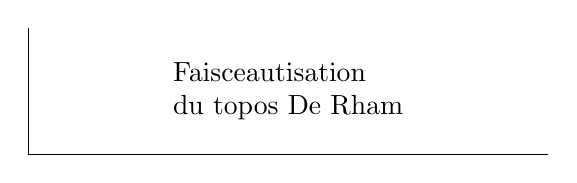
\begin{tikzpicture}
\node[align=left] at (3.3,.6) {Faisceautisation\\du topos De Rham};
\draw (0,1.4)--(0,-.2)--(6.6,-.2);
\end{tikzpicture}}}
1. Soit $X$ un topos, et
\[
\mathbb Z\xrightarrow{u}\Phi
\]
une immersion de $\mathbb Z$ dans un faisceau $\Phi$, tel que

a) $\operatorname{Coker}\Phi$ est $\mathbb Z$-plat

b) Pour tout $i>0$, $\Lambda_{\mathbb Z}^i\Phi$ et $\Gamma_{\mathbb Z}^i\Phi$ sont flasques, et le restent par tensorisation avec tout faisceau abélien.

En particulier, on en conclut \deleted{par récurrence et dévissage} que \deleted{\unsure{si}}
b') Si $i,j\geq0$ et $i+j>0$, alors $\deleted{\unsure{\Lambda}}\Gamma_{\mathbb Z}^i\Phi\otimes\Lambda_{\mathbb Z}^j\Phi$ est flasque.

De b') on conclut \deleted{que}\inserted{(par récurrence et dévissage)}, posant
\[
\operatorname{Coker}i=\Psi
\]
\inserted{que}
$\alpha)$ les $\Gamma_{\mathbb Z}^i\Phi\otimes\Lambda_{\mathbb Z}^j\Psi$ sont flasques pour $i>0$. !

De $\alpha$ on conclut \deleted{\unsure{que}}:

$\beta)$ Posant $K_u^{\bullet\bullet}=\Gamma_{\mathbb Z}^*\Phi\otimes\Lambda_{\mathbb Z}^*\Psi$,
avec l'op. diff. \deleted{\unsure{d}} $d$ compatible aux puissances divisées qui,
sur $\deleted{\unsure{\Gamma^0\otimes\Lambda^1}}\Psi$ est nul et sur $\unsure{\widehat\Phi|\Phi}$ est l'hom canonique $\Phi\longrightarrow\Psi$, et définissant
\[
\mathbb Z\{T\}\longrightarrow H^{*0}(K_u^{**})
\]
par $T\longmapsto1\in\mathbb Z=\operatorname{Ker}(\Phi\xrightarrow{d}\Psi)$,
et prolongeant par la condition d'être compatible aux p.div,
on trouve que $K_u^{\bullet\bullet}$ est une \uline{résolution} de $\mathbb Z\{T\}$.

Utilisant encore a), \inserted{et b)}, on trouve

$\gamma)$ Pour tout faisceau d'anneaux comm. $k$ sur $X$,
$K_{u,k}^{\bullet\bullet}\simeq K_u^{\bullet\bullet}\otimes k
\simeq\Gamma_k^*\Phi_k\otimes\Lambda_k^*\Psi_k$ est une résolution de
$k\{T\}\simeq H^{\bullet0}(K_{u,k}^{\bullet\bullet})$, et les
$\Gamma_k^i\Phi_k\otimes\Lambda_k^j\Psi_k$ sont flasques pour $i>0$.
\margin{79}

\scanpage{81}
On va graduer $K_{u,k}^{\bullet\bullet}$ par a) le degré extérieur venant de
$\Lambda_k^*\Psi_k$ $(\deg_{\mathrm{ext}}\Gamma^i\otimes\Lambda^j=j)$
et b) le \uline{degré total} $i+j$. Ainsi $d$ augmente le degré extérieur par 1,
et invarie le degré total \deleted{\unsure{donc}}
(Le degré complémentaire est $\deg_{\mathrm{comp}}\Gamma^i\otimes\Lambda^j=i$,
il est diminué de 1 par $d$.) Muni du degré total (ou complémentaire)
$K_{u,k}^{\bullet\bullet}$ est une Algèbre graduée sur l'Anneau gradué $k\{T\}$.

\unsure{Conséquence} (de $\unsure{\gamma}$ disons de suite)

\uline{Théorème} Soit
$K^{\bullet\bullet}(X,u,k)=\Gamma(X,K_{u,k}^{\bullet\bullet})$.
Alors on a un hom can (du fait que $K_{u,k}^{\bullet\bullet}$
\deleted{\unsure{H}} est une résolution de $k\{T\}$)
\[
\begin{gathered}
H^{**\deleted{\unsure{*}}}(X,u,k)\overset{\mathrm{dfn}}=
H^{**}(K^{\bullet\bullet}(X,u,k))\\
\longrightarrow H^{**}(X,k\{T\})\\
\simeq H^{**}(X,k)\otimes_{\mathbb Z}\mathbb Z\{T\}
\end{gathered}
\]
et ceci est un isomorphisme pour les bidegrés $(i,j)$ tels que
$\deleted{\unsure{i\leq j}}j\leq i$, tandis que
$H^{i,j}(X,u,k)=0$ (et pour cause) pour $j>i$.

\margin{\figure{\begin{tikzpicture}[x=.65cm,y=.48cm]
\draw (0,4.7)--(0,0)--(5.7,.05);
\draw (0,0) circle(.06);
\fill (1,0) circle(.07); \fill (1,1) circle(.06);
\fill (2,0) circle(.07); \fill (2,1) circle(.065); \fill (2,2) circle(.09);
\fill (3,0) circle(.09); \fill (3,1) circle(.05); \fill (3,2) circle(.09); \fill (3,3) circle(.065);
\fill (4,0) circle(.06); \fill (4,1) circle(.04); \draw (4,2) circle(.06);
\fill (4,3) circle(.065); \fill (4,4) circle(.06);
\end{tikzpicture}}}

\uline{Corollaire plus général.} Soit $f:X\longrightarrow Y$ un morphisme de topos. Alors
\[
f_*K_{u,k}^{\bullet\bullet}\longrightarrow Rf_*(k\{T\})
\simeq Rf_*(k)\otimes_{\mathbb Z}\mathbb Z\{\unsure{T}\}
\]
\margin{80}

\scanpage{82}
est un isomorphisme \inserted{en cohomologie} en bidegré $(i,j)$ avec $j\leq i$,
tandis que la coh. du premier mb est nulle pour $j>i$.

On peut l'exprimer comme un isomorphisme du $1^{\mathrm{er}}$ mb avec un certain,
tronqué du second $\ldots$

\uline{Fonctorialités}\quad a) en $k$, clair

b) \uline{En $u$}\deleted{\unsure{k}} Soit
\[
u':\mathbb Z\longrightarrow\Phi'
\]
une deuxième immersion; S'il existe un hom $\lambda:\Phi\longrightarrow\Phi'$
rendant comm.
\diagram{\begin{tikzcd}[column sep=large]
&\mathbb Z\arrow[dl,"u"']\arrow[dr,"u'"]&\\
\Phi\arrow[rr,"\lambda"]&&\Phi'
\end{tikzcd}}
i.e. $\lambda u=u'$

On en conclut $\unsure{\bar\lambda|\tilde\lambda}:K_u^{\bullet\bullet}-K_{u'}^{\bullet\bullet}$
et $\tilde\lambda_k:K_{u,k}^{\bullet\bullet}-K_{u',k}^{\bullet\bullet}$,
compatible avec ttes les structures, qui est un isom. dans \unsure{telle|toute}
catégorie dérivée, et le reste après application de $\Gamma(X,-)$ ou de $f_*$.

Supposons qu'on ait un autre, soit $\mu$, tel que
\[
\mu u=u'
\]
alors, posant $\mu=\lambda+\unsure{\theta|\Theta}$,
on trouve
\[
\unsure{\theta|\Theta}u=0
\]
\margin{81}

\scanpage{83}
$K^{\bullet\bullet}$\quad Algèbre de DR à p.d. élémentaire

a) Anneau bigradué, \deleted{\unsure{comm.}} alterné pour
\inserted{``deg. ext''} à bidegr. $\geq0$

b) \deleted{\unsure{structure}}
Structure à p.d. sur l'idéal $\sum_{i+j>0}K^{ij}$

c) différentielle d'Anneau gradué (pour le grad ext) ne changeant pas le degré total, et comp. avec p.d.

d) $d:K^{1,0}=\Phi\longrightarrow K^{1,1}\unsure{=|\equiv}\Psi$ est un épi.

e) Posant $k=K^{00}$, $K^{**}$ est l'algèbre \inserted{alternée} à p.d. libre engendrée par $\Phi$ et $\Psi$
i.e.
\[
K^{**}\simeq\Gamma^*\Phi\otimes\Lambda^*\Psi
\]
[Il en résulte que $K^{ij}=0$ si $j>i$.]

f) \deleted{$\Psi$ est $k$-plat} $\Phi$ et $\Psi$ sont $k$-plats
(comme aussi $L=\operatorname{Ker}d=H^{10}(K^{\bullet\bullet})$)

Il résulte déjà de ceci que
\[
H^{*i}(K^{\bullet\bullet})=
\begin{cases}
\Gamma^*L&\text{si }i=0\\
0&\text{si }i>0
\end{cases}
\]
donc que $K^{\bullet\bullet}$ est une résolution de $\Gamma^*L$.
On va supposer le plus souvent

g) $L$ est un $k$-Module \deleted{\unsure{inversible}}\inserted{loc. lib. de rang 1}.
(Voire libre de rang 1 et trivialisé $\ldots$)
\margin{82}

\scanpage{84}
UNIVERSITE DES SCIENCES ET TECHNIQUES\\
DU LANGUEDOC\\
Mathématiques
\margin{MONTPELLIER, le 10 juillet 1975}

\uline{JOURNEES MATHEMATIQUES S.M.F.}

``Formes quadratiques et questions connexes''

18 au 22 novembre 1975

(1ère annonce)

A l'heure actuelle, les conférenciers suivants ont accepté de participer à ces journées d'études :

H. GROSS, Mathematisches Institut der Universität Zurich

Formes quadratiques et sesquilinéaires dans les espaces de dimension infinie.

A. FROHLICH, University of London

Hermitian class group of integral group rings and arithmetic applications.

W. SCHARLAU, Mathematisches Institut der Universität Münster

Quadratic forms in additive categories (titre provisoire)

A. GRAMAIN, Université de Tours

Titre non parvenu.

O. LABORDE, Université de MONTPELLIER

\unsure{Classes} caractéristiques d'un module quadratique en cohomologie étale.

Mme C. HØSTMAELINGEN, Université d'Oslo

Anneaux de Witt des anneaux de Prüfer.

A. MICALI et Ph REVOY, Université de \unsure{Montpellier}

Sur l'existence de produits vectoriels et variétés de Stiefel algébriques.

Pour tout renseignement concernant ce colloque, vous êtes priés de vous adresser à :

Mme P. ARNAUD\\
Secrétaire de l'U.E.\unsure{R}. de Mathématiques\\
Université des Sciences et Techniques du Languedoc\\
Place Eugène Bataillon\\
34060 MONTPELLIER CEDEX

\figure{\begin{tikzpicture}\draw (0,0)--(2.5,0);\end{tikzpicture}}
\margin{83}

\scanpage{85}
\deleted{Soient $K^{\cdot\cdot}$ et $K'^{\cdot\cdot}$.}

Finalement, la donnée de $K^{\cdot\cdot}$ équivaut à celle de

$\alpha)$ $k$, Anneau comm. sur $X$

$\beta)$ $L$, $k$-Module plat (voire inversible voire $k$ lui-$=$\ldots)

$\gamma)$ Une immersion de $L$ dans un $k$-module $\Phi$, $u:L\mathbin{-}\Phi$.

Soit de $\unsure{=|\mathrm{m.}}$ $K'^{\cdot\cdot}$ défini par $(k',L',\Phi',u')$. \deleted{\unsure{ou}} La donnée d'un hom $\lambda$ de $K^{\cdot\cdot}$ dans $K'^{\cdot\cdot}$, compatible avec ttes les structures, équivaut à la donnée d'un syst. d'hom

\diagram{\begin{tikzcd}
k \arrow[r,"\deleted{\unsure{\lambda}}\lambda_0"] & k'
\end{tikzcd}}
hom d'Anneaux

\deleted{\diagram{\begin{tikzcd}
L \arrow[r,"\unsure{\lambda_L}"] & L'
\end{tikzcd}}}

\diagram{\begin{tikzcd}
\Phi \arrow[r,"\lambda_\Phi",dash] & \Phi'
\end{tikzcd}}
$\left\{\text{hom $\lambda_0$-}\unsure{\tfrac12\text{ linéaire}|k\text{ linéaire}}\right.$
\deleted{\unsure{ou}}

avec $\lambda_\Phi(u(L))\subset u'(L')$, donc $\lambda_\Phi$
\deleted{\illegible{4}}
induit un hom (évidemment $\lambda_0$-$\frac12$ lin.)
\deleted{\diagram{\begin{tikzcd}
L \arrow[r,"\unsure{\lambda} ",dash] \arrow[d] & L' \arrow[d] \\
\Phi \arrow[r,dash] & \Phi'
\end{tikzcd}}}
\diagram{\begin{tikzcd}
L \arrow[r,"\lambda_L"] & L'
\end{tikzcd}}

Dans le cas $L\simeq k$, $L'\simeq k'$ donnés, on peut oublier $L,L'$ et \unsure{retenir} $\Phi,\Phi'$ avec sections marquées, et la condition sur $\lambda_\Phi$

\margin{84}

\scanpage{86}
UNIVERSITE DES SCIENCES\\
ET TECHNIQUES DU LANGUEDOC

\figure{\begin{tikzpicture}\draw[dashed] (0,0)--(2,0);\end{tikzpicture}}

Service de la Scolarité\\
AMC/GJ

Montpellier, le 17 Juillet 1975

\uline{Diffusion :} Liste H\\
N°4617

AVIS DE SOUTENANCE\\
D'UNE THESE DE DOCTORAT D'ETAT

\figure{\begin{tikzpicture}\draw (0,0)--(2.4,0);\end{tikzpicture}}

\uline{Nom et prénom du candidat} : FOLLET Michel

\uline{Titre de la Thèse} : Etude physicochimique de la réactivité du cycle triazine : Synthèse et analyse spectrale de dérivés bicycliques.

\uline{Date, heure et lieu de soutenance prévus} :\\
8 Septembre 1975 à 17 Heures,\\
Salle de cours n° 9.

\uline{Nom du Directeur de thèse} : Professeur JACQUIER.

\uline{Désignation du laboratoire où la thèse est préparée} : Laboratoire de Synthèse et d'Etude Physicochimique d'Hétérocycles Azotés.

\uline{Résumé de la thèse} : Ce travail porte sur la série de la triazine - 1,2,4 , plus particulièrement sur les dérivés de l'acide thioxo-3 oxo-5 tétrahydro-2,3,4,5 triazine carboxylique -6. Différentes méthodes de synthèse de triazolo-triazines et triazolyl - triazines sont données. L'analyse spectrale de ces composés est faite par UV, RMN et spectrométrie de masse.

\uline{Durée approximative des recherches ayant abouti à la thèse} : 4 ans.

\uline{Noms des rapporteurs} :

JACQUIER R., Professeur, Chimie organique, U.S.T.L.\\
GRANGER R., Professeur, Chimie organique; Université MONTPELLIER I.\\
VIALLEFONT Ph. Professeur, Chimie organique, U.S.T.L.

\uline{Composition du jury} :

JACQUIER R., Professeur, Chimie organique, U.S.T.L. (Président)

GRANGER R., Professeur, Chimie organique, Université MONTPELLIER I (Membre extérieur choisi en raison de sa compétence scientifique)

DESCHAMPS J. Professeur, Chimie-physique, Faculté de Pau et des Pays de l'Adour (Membre étranger à la spécialité du candidat)

VIALLEFONT Ph. Professeur, Chimie organique, U.S.T.L.

DAUNIS J., Chargé de Recherche CNRS, Chimie organique, U.S.T.L.

LE SECRETAIRE GENERAL

\figure{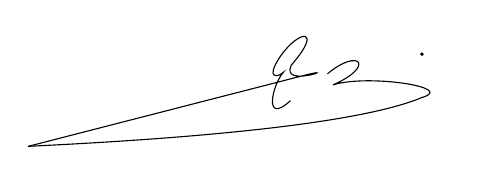
\begin{tikzpicture}[x=1cm,y=1cm]
\draw (0,0)--(3.5,.9) .. controls (4,1.03) and (3.2,.73) .. (3.34,1.03)
.. controls (3.75,1.5) and (3.45,1.5) .. (3.2,1.14)
.. controls (3,.84) and (3.18,.88) .. (3.24,.94)
.. controls (3.1,.78) and (2.98,.26) .. (3.33,.58);
\draw (3.8,.92) .. controls (4.2,1.26) and (4.42,1.02) .. (3.87,.78)
.. controls (4.3,.92) and (5.45,.75) .. (5,.62)
.. controls (4,.2) and (1,.05) .. (0,0);
\fill (5,1.17) circle (.025);
\end{tikzpicture}}

\uline{E. SIAU}

MR LE PROFESSEUR GROTHENDIECK A.\\
MATHEMATIQUES\hfill 5-856

\margin{85}

\scanpage{87}
devient donc de transformer section marquée en section marquée.

Supposons que nous ayons deux hom $\lambda,\mu$, correspondant à un \uuline{$=$} homom.
\diagram{\begin{tikzcd}
k \arrow[r,"\lambda_0=\mu_0"] & k'
\end{tikzcd}}
et deux hom
\diagram{\begin{tikzcd}
\Phi \arrow[r,shift left=.4ex,"{\lambda_\Phi,\mu_\Phi}"] \arrow[r,shift right=.4ex] & \Phi'
\end{tikzcd}}
(ayant $=$ effet sur la section marquée).
Que peut-on dire des hom $\lambda,\mu$ de $K^{\cdot\cdot}$ dans $K'^{\cdot\cdot}$ ?

\margin{\figure{\begin{tikzpicture}\draw (0,0)--(.10,.18);\end{tikzpicture}}}
\margin{86}

\scanpage{88}
U N I V E R S I T E\\
DES SCIENCES ET TECHNIQUES\\
DU LANGUEDOC

\figure{\begin{tikzpicture}\draw[dashed] (0,0)--(2,0);\end{tikzpicture}}

AMC/GJ\\
\uline{Diffusion} : Liste A\\
N°4549

Montpellier, le 16 Juillet 1975

\uline{AVIS DE SOUTENANCE D'UNE THESE DE DOCTEUR-INGENIEUR}

\uline{Nom et prénom du candidat} : DASSOUKI Mouhiddine

\uline{Titre de la thèse} : Etude expérimentale et théorique d'une machine à courant continu à commutation par thyristors tournant avec l'induit.

\uline{Date, heure et lieu de soutenance prévus} :\\
29 Juillet 1975 à 10 Heures\\
Salle de cours n° 9.

\uline{Nom du Directeur de thèse} : R. JOUTY

\uline{Désignation du laboratoire où la thèse est préparée} : Laboratoire de Physique des Métaux.

\uline{Analyse de l'ouvrage} : Il est possible de remplacer le collecteur d'une machine à courant continu classique par une batterie de thyristors. Pour la commande de ces derniers, leurs gachettes sont reliées à un collecteur auxiliaire. L'étude de ce type nouveau de machine fait apparaître des similitudes, mais aussi de grandes différences avec la machine classique; notamment en ce qui concerne la commutation et la réaction d'induit, dont l'auteur donne une analyse très détaillée. L'étude expérimentale, faite sur un prototype obtenu par transformation d'une machine classique, est en bon accord avec la théorie, et fait apparaître des performances satisfaisantes.

\uline{Durée approximative des recherches ayant abouti à la thèse} : 2 ans.

\uline{Composition du jury proposé} :

Monsieur JOUTY R.\\
Monsieur GROUBERT E.\\
Monsieur TROMPETTE

LE SECRETAIRE GENERAL,

\figure{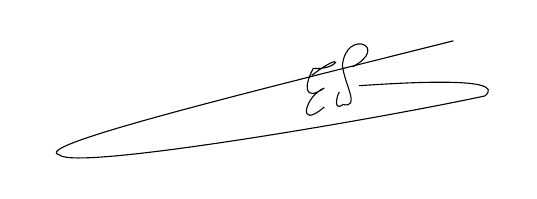
\begin{tikzpicture}[x=1cm,y=1cm]
\draw (5,1.45) .. controls (2,.7) and (-.4,.1) .. (0,0)
.. controls (.2,-.2) and (4,.45) .. (5.4,.75)
.. controls (5.7,1) and (4.4,.92) .. (3.8,.88);
\draw (3.2,1.01) .. controls (3.65,1.36) and (3.55,1.07) .. (3.22,1.1)
.. controls (3.1,.88) and (3.1,.67) .. (3.36,.85)
.. controls (3.12,.76) and (3.0,.3) .. (3.36,.61);
\draw (3.72,1.12) .. controls (4.2,1.38) and (3.64,1.61) .. (3.59,1.14)
.. controls (3.62,.88) and (3.82,.6) .. (3.6,.64)
.. controls (3.47,.55) and (3.52,.75) .. (3.55,.8);
\end{tikzpicture}}

\uline{E. SIAU}

\margin{87}

\scanpage{89}
$X$, topos\\
$k$ Anneau sur $X$

$k\overset{u}{\hookrightarrow}\Phi$ mono dans $k$-Module, avec
\[
\left\{\begin{array}{ll}
\text{\textcircled{a}}&\Psi=\operatorname{Coker}u\quad k\text{-plat}\\
\text{\textcircled{b}}&\forall\ k\text{-modules }M,N,\text{ et }i>0\\
&\Gamma^i(N\otimes_k\Phi)\otimes M\longrightarrow\text{flasque}
\end{array}\right.
\]

\uline{Lemme} $\forall$ $k$-modules $\unsure{S|B}$, $\exists$ \deleted{hom} $S\overset{u_S}{\longrightarrow}\unsure{\widetilde N|\overleftarrow N}$, qui \textcircled{a} est un $k$-mono ``universel'' (reste mono par tensorisation) tel que $\unsure{S|N}$ plat $\Rightarrow$ $\operatorname{Coker}\unsure{u_N|u_S}$ plat, et \textcircled{b'} $\forall i>0$, et $k$ modules $\unsure{N|P},M$
\[
\Gamma_k^i(\widetilde N\otimes_k P)\otimes_k M\quad\text{flasque}
\]

\margin{\figure{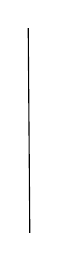
\begin{tikzpicture}\draw (0,0)--(.02,-2.6);\end{tikzpicture}}}

On prend $\widetilde N=\unsure{\Phi}\otimes_k\unsure{S|B}$, $u_S=u\otimes\operatorname{id}_S$, d'où a) résulte de a), et b') de b).

\[
\mathcal{DR}_{pd}^{**}(\deleted{\unsure{k,\Phi}}k,u)
=\Gamma^*(\unsure{\Psi|\Phi})\otimes_k\Lambda^*\Psi
\]
Anneau bigradué (degré compl. + degré ext. = degré total)
\inserted{alterné pour deg. ext.}
différentiel à p.d. (sur idéal des \unsure{bidegrés} $>0\unsure{\ldots}$) une résolution de $k\{T\}$. (où deg ext $T=0$, deg tot $T=1$)
\[
\mathrm{DR}_{pd}^{**}(k,u)=\Gamma(X,\mathcal{DR}_{pd}^{**}(k,u)).
\]

Soit $\mathbb{DR}^{**}$ la cat \inserted{\uline{dérivée}} des anneaux bigradués (à deg $\geq0$) alternés diff. à p.d., \inserted{avec \unsure{un $T$ élémt marqué} pur bidegré $(1,0)$} on \unsure{définit} un syst. transitif d'isom. dans $\mathbb{DR}^{**}$ entre les $\mathrm{DR}_{pd}^{**}(k,u)$, pour $k$ fixé et $u$ variable.

Notons que si on a
\diagram{\begin{tikzcd}
&\Phi \arrow[dd,"\lambda"]\\
k \arrow[ur,"u"] \arrow[dr,"u'"',dash]&\\
&\Phi'
\end{tikzcd}}
d'où
$\lambda^{**}:\mathrm{DR}_{pd}^{**}(k,u)\mathbin{-}\mathrm{DR}_{pd}^{**}(k,u')$,
donc $\lambda^{**}$ est un iso. dans $\mathbb{DR}^{**}$.

\unsure{\diagram{\begin{tikzcd}
&\Phi' \arrow[dr,hook]& &\\
k \arrow[ur,hook,"u"] \arrow[dr,hook,"u'"']&&S \arrow[r,hook,"\text{donné par lemme}"] \arrow[d,equal]&N\\
&\Phi \arrow[ur,hook] &\Phi\amalg_k\Phi'&
\end{tikzcd}}}

d'où
\diagram{\begin{tikzcd}
\mathrm{DR}(u)\arrow[dr,"\sim"]&\\
&\mathrm{DR}(N)\\
\mathrm{DR}(u')\arrow[ur,"\sim"]&
\end{tikzcd}}
d'où $\mathrm{DR}(u)\simeq\unsure{\mathrm{DR}(u')}$ dans $\mathbb{DR}^{**}$

indépendant du choix de $S\hookrightarrow N$ avec $N$ comme dans le lemme
\unsure{\diagram{\begin{tikzcd}
&N \arrow[dr,hook]&&\\
S \arrow[ur,hook] \arrow[dr,hook]&&T \arrow[r,hook,"\text{donné par lemme}"]\arrow[d,equal]&N''\\
&N' \arrow[ur,hook]&N\amalg_S N'&
\end{tikzcd}}}
\margin{$k$}
d'où
\diagram{\begin{tikzcd}
\mathrm{DR}(u)\arrow[dr]&&\mathrm{DR}(N)\arrow[dr,"\sim"]&\\
&\mathrm{DR}(S)\arrow[ur]\arrow[dr]&&\mathrm{DR}(N''\qquad\sim\\
\mathrm{DR}(u')\arrow[ur]&&\mathrm{DR}(N')\arrow[ur,"\sim"]&
\end{tikzcd}}

Transitivité évidente par \unsure{diagramme}.

\margin{88}

\scanpage{90}
\margin{- 175 -}
\margin{IX}

(13.3.15)
\diagram{\begin{tikzcd}
0 \arrow[r] & R^f/R^t \arrow[r] & E/E^t \arrow[r] & B \arrow[r] & 0
\end{tikzcd}}
.

On notera que
\[
\text{(13.3.16)}\qquad R^f/R^t=(R_o/R_o^t)_S
\]
est un groupe analytique constant sur $S$. Il résulte donc de 13.1.5 que $B$ est un groupe abéloïde sur $S$ au voisinage de $s$ si et seulement si sa fibre en $s$
\[
B_o=A_o/T_o
\]
est un groupe analytique abéloïde, de sorte que $A_o$ apparaît alors comme une extension d'un tel groupe $B_o$ par un tore $T_o$. \uline{Toute façon d'écrire} $A_o$ \uline{sous forme d'une extension d'un groupe abéloïde par un tore complexe} (*) \uline{donne donc naissance sur} $A$, \uline{au voisinage de} $s$, \uline{à une unique structure d'extension} (13.3.13) \uline{d'un groupe abéloïde} $B$ \uline{par un tore} $T$, \uline{induisant la structure d'extension donnée en} $s$.

13.4. \uline{Interprétation en termes de} ``\uline{structures de Hodge mixtes}'' \uline{de DELIGNE}.

Reprenons d'abord le dictionnaire 13.1.4, que nous allons reformuler d'une façon légèrement différente, mieux adaptée à l'introduction des ``structures de Hodge'' pertinentes à la situation. Pour ceci, soit $\mathbb R$ le faisceau des sections de $R$ sur $S$, et introduisons le $\underline O_S$-Module
\[
\text{(13.4.1)}\qquad \mathcal E(A)=\mathcal E=\underline R\otimes_{\mathbb Z}\underline O_S,
\]
qui est localement libre de type fini lorsque $R$ est localement constant. (NB Le faisceau $\mathcal E$ n'est pas nécessairement cohérent si $R$ n'est pas localement constant.) L'homomorphisme (13.1.3) $\underline R\longrightarrow\underline E$ définit alors

\margin{\unsure{493|1493}}
\margin{493}
\margin{89}

\scanpage{91}
\diagram{\begin{tikzcd}[column sep=small,row sep=small]
&\Phi \arrow[r,dash]&N \arrow[ddr,dash]&\\
k \arrow[ur,"u"]\arrow[r,dash,"u'"]\arrow[dddr,"u''"']&\Phi' \arrow[ur,dash]\arrow[dddr,dash]&&\\
&\deleted{\unsure{\Phi'}}\arrow[ul,dash,"\deleted{\unsure{u'}}"]&&N''\\
&&&\\
&\Phi''\arrow[r,dash]&N'\arrow[uur,dash]&
\end{tikzcd}}

d'où
\diagram{\begin{tikzcd}
&\Phi\arrow[dr]&\\
k\arrow[ur]\arrow[r]\arrow[dr]&\Phi'\arrow[r]&N''\\
&\Phi''\arrow[ur]&
\end{tikzcd}}
\diagram{\begin{tikzcd}
\mathrm{DR}(\Phi)\arrow[dr,"\sim"]&\\
\mathrm{DR}(\Phi')\arrow[r,"\sim"]&\mathrm{DR}(N'')\\
\mathrm{DR}(\Phi'')\arrow[ur,"\sim"]&
\end{tikzcd}}

Argument analogue pour $f_*(\mathcal{DR}_{pd}^{**}(k,u))$, si $f:X\mathbin{-}Y$ morphisme de topos.

\uline{Condition} de \uline{De Rham sur Anneau} $k$ : la condition d'existence d'un $u:k\mathbin{-}\Phi$ tel que\ldots

Si $k$ satisfait condition de De Rham, de $=$ tte $k$-Algèbre. \unsure{Donc|Dans} le plus beau, c'est que $\mathbb Z_X$ y satisfasse ! C'est vrai pour

a) le topos ss $\widehat\Delta$

b) le topos défini par un espace topologique. \unsure{Voir cours ant.}

\uline{Question} Est-ce vrai pour $\widehat{\Delta^\circ}$ (topos des ens. cosimpliciaux) ? \uuline{\uline{Non}}

Soit $A^{**}\in\operatorname{Ob}\mathbb{DR}_{pd}^{**}(X)$ une Algèbre bigraduée à degrés positifs, alternée pour le degré ext., diff. à p. div.\ldots Supposons que $A^{00}=k$ satisfasse la condition de De Rham, soit $u:k\mathbin{-}\Phi$ d'où $\mathcal{DR}_{pd}^{**}(k,u)$. Considérons alors
\[
\overline A^{**}\unsure{=|.}\mathcal{DR}_{pd}^{**}(A^{**})
\overset{\mathrm{dfn}}=
\mathcal{DR}_{pd}^{**}(k,\unsure{u})\otimes_{k\{T\}}A^{**},
\]
l'augmentation
\[
k\{T\}\mathbin{-}\mathcal{DR}_{pd}^{\unsure{**|*}}(\unsure{k,u})
\]
\inserted{(qui est un quasi-iso \uline{universel})}
définit un hom
\diagram{\begin{tikzcd}
A^{**}\arrow[r]&\overline A^{**}
\end{tikzcd}}
qui est un quasi-iso.
\deleted{\unsure{D'après}}
\inserted{En effet}

\margin{90}

\scanpage{92}
\margin{- 174 -}
\margin{IX}

(13.3.9) correspond simplement à l'homomorphisme
\[
E^t/R_{oS}^t=E^t/R^t\longrightarrow E/R_{oS}=E/R^f
\]
induit par les inclusions
\[
E^t\hookrightarrow E,\quad R^t\hookrightarrow R^f.
\]

Utilisant le fait que (13.3.9) induit une immersion sur les fibres en $s$, on en conclut que l'homomorphisme
\[
R_o/R_o^t\longrightarrow E_o/E_o^t=(E/E^t)_o
\]
est injectif, d'où il résulte aussitôt que
\[
R_o/R_o^t\longrightarrow(E/E^t)_{s'}
\]
est encore injectif pour $s'$ voisin de $s$, ce qui implique que, quitte à rapetisser $S$ autour de $s$, on peut supposer que (13.3.9) \uline{est une immersion fermée}.

Il s'impose alors d'introduire
\[
\text{(13.3.12)}\qquad B=A^\natural/T\simeq(E/E^t)/(R^f/R^t),
\]
de sorte qu'on obtient sur $A^\natural$ une structure d'extension

(13.3.13)
\diagram{\begin{tikzcd}
0\arrow[r]&T\arrow[r]&A^\natural\arrow[r]&B\arrow[r]&0
\end{tikzcd}}
,

$B$ étant un groupe analytique relatif sur $S$, lisse et séparé sur $S$ et à fibres connexes. Par construction même, on a donc
\[
\text{(13.3.14)}\qquad \underline{\operatorname{Lie}}(B)\simeq\underline E/\underline E^t,
\]
et la suite exacte exponentielle pour $B$

\margin{\unsure{492}}
\margin{492}
\margin{91}

\scanpage{93}
\margin{92}

\scanpage{94}
\deleted{(à p. div. \unsure{sous})}

\margin{\figure{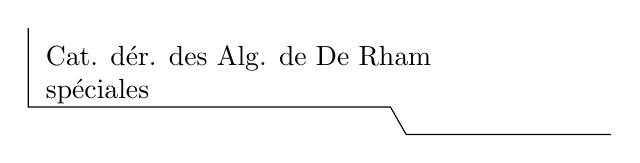
\begin{tikzpicture}
\node[anchor=west,align=left] at (.1,.4) {Cat. dér. des Alg. de De Rham\\spéciales};
\draw (0,1)--(0,0)--(4.6,0)--(4.8,-.35)--(7.4,-.35);
\end{tikzpicture}}}

Structure De Rham (à p.d. - sous-entendus)

Anneau bigradué [à degrés - total et ext - $\geq0$]\\
alterné pour degré ext
\[
A^{ij}\neq0\quad\deleted{\unsure{\Leftarrow}}\Rightarrow\unsure{q|0}\leq j\leq i
\]
degré complémentaire $=\unsure{j|i}-j\geq0$

différentiel [différentielle de bidegré $0,1$ ; c'est un diff. pour le degré ext $\unsure{j}$
\[
d(xy)=(dx)y+(-1)^{\deg.\mathrm{ext}\,x}x\,dy
\]
]

à p. div. sur l'idéal
\[
\sum_{i+j>0}A^{ij}=A^+
\]
[p.d. \deleted{\unsure{divisées}} compatibles aux $2$ grad
$\bigl(\gamma^d:A^{ij}\mathbin{-}A^{di,dj}\bigr)$
\deleted{\unsure{d}}
et la différentielle $(d\,x^{(i)}=x^{(i-1)}\,dx)$]

élément \uline{marqué}
$T\in Z^{10}(A^{**})\simeq H^{10}(A^{**})$

[Cohomologie $H^{*i}(A^{**})\simeq\unsure{h^i|h_i^i}\otimes_k k\{T\}$, \deleted{\unsure{où}}] $k=A^{00}$

Structure de De Rham \uline{spéciale} :
\[
\left\{\begin{array}{l}
k\{T\}\overset{\sim}{\longrightarrow}H^{*0}(A^{**})\\
H^{*i}(A^{**})=0\\
\text{les }A^{ij}\text{ sont }k\text{-plats}
\end{array}\right.
\]
[\uline{NB} c'est utile pour la stabilité par $\otimes_k k'$]

Structure de De Rham \uline{flasque} : les $A^{ij}$ pour $j<i$

\margin{$\unsure{)}\longrightarrow$ flasques.}
\margin{Univ. flasque : \deleted{stabilité par $\otimes_k\unsure{k'}$}}
\margin{\figure{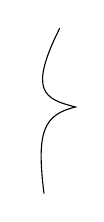
\begin{tikzpicture}
\draw (.2,1)..controls(-.2,.2)and(0,.1)..(.4,0)
..controls(0,-.1)and(-.1,-.3)..(0,-1.1);
\end{tikzpicture}}}

On parle de $k$-Structure de De Rham si $k=A^{00}$ \unsure{$\longrightarrow$|est} donné.

\deleted{$\unsure{\mathcal X}$}
$\mathcal X$, topos

\deleted{$\unsure{\mathcal{DR}}$}
$\mathcal{DR}_{sp}(\mathcal X,k)_0$ structures de De Rham spéciales sur $\mathcal X$ - avec comme flèches celles qui respectent \unsure{toutes|ttes} les structures \inserted{(y compris la structure $\unsure{u|k}$)}

$\mathcal{DR}_{spfl}(\mathcal X,\unsure{k})_0$ \quad `` \quad spéciales et flasques

$\mathcal{DR}_{spufl}(\mathcal X,\unsure{k})_0$ \quad `` \quad --- univ. flasques

$\mathcal{DR}_{sp}(\mathcal X,k)$, $\mathcal{DR}_{spfl}(\mathcal X,k)$, $\mathcal{DR}_{spufl}(\mathcal X,k)$

Catégories \inserted{de fractions} déduites en rendant inversibles ttes les flèches

- NB ce sont des quasi-isos -

\margin{93}

